%#!uplatex
%%%%%%%%%%%%%%%%%%%%%%%%%%%%%%%%%%%%%%%%%%%%%%%%%%%%%%%%%%%%%%%%%%%%%%%%%%%%%%%%%%%%%%%%%%%%%%%%%%%
%%%%%%%%%%%%%%%%%%%%%%%%%%%%%%%%%%%%%%%%%%%%%%%%%%%%%%%%%%%%%%%%%%%%%%%%%%%%%%%%%%%%%%%%%%%%%%%%%%%
%%%%%%%%%%%%%%%%%%%%%%%%%%%%%%%%%%%%%%%%%%%%%%%%%%%%%%%%%%%%%%%%%%%%%%%%%%%%%%%%%%%%%%%%%%%%%%%%%%%
\documentclass[12pt,dvipdfmx,uplatex]{beamer}
%%%%%%%%%%%%%%%%%%%%%%%%%%%%%%%%%%%%%%%%%%%%%%%%%%%%%%%%%%%%%%%%%%%%%%%%%%%%%%%%%%%%%%%%%%%%%%%%%%%
%%%%%%%%%%%%%%%%%%%%%%%%%%%%%%%%%%%%%%%%%%%%%%%%%%%%%%%%%%%%%%%%%%%%%%%%%%%%%%%%%%%%%%%%%%%%%%%%%%%
%%%%%%%%%%%%%%%%%%%%%%%%%%%%%%%%%%%%%%%%%%%%%%%%%%%%%%%%%%%%%%%%%%%%%%%%%%%%%%%%%%%%%%%%%%%%%%%%%%%
%%%
%%% hyperref 文字化け対策
%%%
\usepackage{pxjahyper}
\usepackage{hyperref}
%%%%%%%%%%%%%%%%%%%%%%%%%%%%%%%%%%%%%%%%%%%%%%%%%%%%%%%%%%%%%%%%%%%%%%%%%%%%%%%%%%%%%%%%%%%%%%%%%%%
%%%%%%%%%%%%%%%%%%%%%%%%%%%%%%%%%%%%%%%%%%%%%%%%%%%%%%%%%%%%%%%%%%%%%%%%%%%%%%%%%%%%%%%%%%%%%%%%%%%
%%%%%%%%%%%%%%%%%%%%%%%%%%%%%%%%%%%%%%%%%%%%%%%%%%%%%%%%%%%%%%%%%%%%%%%%%%%%%%%%%%%%%%%%%%%%%%%%%%%
%%%
%%% 各種パッケージ
%%%
\usepackage{graphicx}
%\usepackage{url,cite}
\usepackage{amsmath}
\usepackage{amsthm} \theoremstyle{definition} %theorem環境が斜体になるので注意
\usepackage{amssymb} % AMS-TeX
\usepackage{setspace}
\usepackage{multirow}
\usepackage{udline} % udline.sty

%%%%%%%%%%%%%%%%%%%%%%%%%%%%%%%%%%%%%%%%%%%%%%%%%%%%%%%%%%%%%%%%%%%%%%%%%%%%%%%%%%%%%%%%%%%%%%%%%%%
%%%%%%%%%%%%%%%%%%%%%%%%%%%%%%%%%%%%%%%%%%%%%%%%%%%%%%%%%%%%%%%%%%%%%%%%%%%%%%%%%%%%%%%%%%%%%%%%%%%
%%%%%%%%%%%%%%%%%%%%%%%%%%%%%%%%%%%%%%%%%%%%%%%%%%%%%%%%%%%%%%%%%%%%%%%%%%%%%%%%%%%%%%%%%%%%%%%%%%%
%%%
%%% 本文・数式フォント
%%%
\usepackage{newtxtext}
\usepackage[varg]{newtxmath}
%\usepackage{newpxtext}
%\usepackage[varg]{newpxmath}

% \mathcal(\cal)の扱い
%\DeclareMathAlphabet{\mathcal}{OMS}{cmsy}{m}{n} %computer modern
%\DeclareMathAlphabet{\mathcal}{OMS}{txsy}{m}{n} %txfont
%\usepackage[psamsfonts]{eucal} % euler

% mathptmx時に数式モードのvをtxfontから借りる
% \DeclareSymbolFont{lettersA}{U}{txmia}{m}{it}
% \SetSymbolFont{lettersA}{bold}{U}{txmia}{bx}{it}
% \DeclareFontSubstitution{U}{txmia}{m}{it}
% \DeclareMathSymbol{v}{\mathalpha}{lettersA}{"33} %"

%%%%%%%%%%%%%%%%%%%%%%%%%%%%%%%%%%%%%%%%%%%%%%%%%%%%%%%%%%%%%%%%%%%%%%%%%%%%%%%%%%%%%%%%%%%%%%%%%%%
%%%%%%%%%%%%%%%%%%%%%%%%%%%%%%%%%%%%%%%%%%%%%%%%%%%%%%%%%%%%%%%%%%%%%%%%%%%%%%%%%%%%%%%%%%%%%%%%%%%
%%%%%%%%%%%%%%%%%%%%%%%%%%%%%%%%%%%%%%%%%%%%%%%%%%%%%%%%%%%%%%%%%%%%%%%%%%%%%%%%%%%%%%%%%%%%%%%%%%%
%%%
%%%  日本語フォントをゴシックに、数式フォントを太字に変更する
%%%
\usepackage[deluxe]{otf}
\renewcommand{\kanjifamilydefault}{\gtdefault}
\renewcommand{\familydefault}{\sfdefault}

\setbeamerfont{title}{size=\large,series=\bfseries}
\setbeamerfont{frametitle}{size=\large,series=\bfseries}
%\setbeamertemplate{frametitle}[default][center]
\usefonttheme{professionalfonts} 

%%%
% Suppress Warning in the case of uplatex
\DeclareFontShape{JY2}{hgt}{b}{n}{<->ssub*hgt/bx/n}{}
\DeclareFontShape{JT2}{hgt}{b}{n}{<->ssub*hgt/bx/n}{}

%\mathversion{bold} %数式フォントを太字に

%%%%%%%%%%%%%%%%%%%%%%%%%%%%%%%%%%%%%%%%%%%%%%%%%%%%%%%%%%%%%%%%%%%%%%%%%%%%%%%%%%%%%%%%%%%%%%%%%%%%%%
%%% Beamer template preamble
%%%
%%% �ơ��ޤλ��ꡢ��ά���� default �ˤʤ�
%%%

 % �ե졼��λ��ꡢ��ά��
%%%%%%%%%%%%%%%%%%%%%%%%%%%% THEME
  %\usetheme{AnnArbor}
  %\usetheme{Antibes}
  %\usetheme{Bergen}
  %\usetheme{Berkeley}
  %\usetheme{Berlin}
  \usetheme{Boadilla}
  %\usetheme{boxes}
  %\usetheme{CambridgeUS}
  %\usetheme{Copenhagen}
  %\usetheme{Darmstadt}
  %\usetheme{default}
  %\usetheme{Dresden}
  %\usetheme{Frankfurt}
  %\usetheme{Goettingen}
  %\usetheme{Hannover}
  %\usetheme{Ilmenau}
  %\usetheme{JuanLesPins}
  %\usetheme{Luebeck}
  %\usetheme{Madrid}
  %\usetheme{Malmoe}
  %\usetheme{Marburg}
  %\usetheme{Montpellier}
  %\usetheme{PaloAlto}
  %\usetheme{Pittsburgh}
  %\usetheme{Rochester}
  %\usetheme{Singapore}
  %\usetheme{Szeged}
  %\usetheme{Warsaw}

% ����
%%%%%%%%%%%%%%%%%%%%%%%%%%%% COLOR THEME
  %\usecolortheme{albatross}
  %\usecolortheme{beetle}
  %\usecolortheme{crane}
  %\usecolortheme{default}
  %\usecolortheme{dolphin}
  %\usecolortheme{dove}
  %\usecolortheme{fly}
  %\usecolortheme{lily}
  %\usecolortheme{orchid}
  %\usecolortheme{rose}
  %\usecolortheme{seagull}
  %\usecolortheme{seahorse}
  %\usecolortheme{sidebartab}
  %\usecolortheme{structure}
  %\usecolortheme{whale}

% �إå����եå����ե졼��������ꡢ��ά��
  %%%%%%%%%%%%%%%%%%%%%%%%%%%% OUTER THEME
  %\useoutertheme{default}
  %\useoutertheme{infolines}
  %\useoutertheme{miniframes}
  %\useoutertheme{shadow}
  %\useoutertheme{sidebar}
  %\useoutertheme{smoothbars}
  %\useoutertheme{smoothtree}
  %\useoutertheme{split}
  %\useoutertheme{tree}

% �����ȥ롢section, itemize/enumerate �Ķ���
% theorem �Ķ�����, ����ʸ���ʤɤΥ����������ꡢ
% ����
  %%%%%%%%%%%%%%%%%%%%%%%%%%%% INNER THEME
  %\useinnertheme{circles}
  %\useinnertheme{default}
  %\useinnertheme{inmargin}
  \useinnertheme{rectangles}
  %\useinnertheme{rounded}


%\usefonttheme{}	% ����
%\logo{}		% ����
%\logo{\includegraphics[width=2cm]{titech_logo.eps}}

% navi. symbols����Ω���ʤ�����dvipdfmx��Ȥ��ȵ�ǽ���ʤ��Τ���ɽ����
\setbeamertemplate{navigation symbols}{}
%\setbeamertemplate{caption}[numbered]
%%%%%%%%%%%%%%%%%%%%%%%%%%%%%%%%%%%%%%%%%%%%%%%%%%%%%%%%%%%%%%%%%%%%%%%%%%%%%%%%%%%%%%%%%%%%%%%%%%%
%%%%%%%%%%%%%%%%%%%%%%%%%%%%%%%%%%%%%%%%%%%%%%%%%%%%%%%%%%%%%%%%%%%%%%%%%%%%%%%%%%%%%%%%%%%%%%%%%%%
%%%%%%%%%%%%%%%%%%%%%%%%%%%%%%%%%%%%%%%%%%%%%%%%%%%%%%%%%%%%%%%%%%%%%%%%%%%%%%%%%%%%%%%%%%%%%%%%%%%

% \AtBeginSection[] % Do nothing for \section*
% { \begin{frame}<beamer> \frametitle{}
%    \tableofcontents[currentsection,subsectionstyle=hide]
%  \end{frame} } 

%appendix��ڡ���������Ȥ��ʤ�
\newcommand{\backupbegin}{
   \newcounter{framenumberappendix}
   \setcounter{framenumberappendix}{\value{framenumber}}
}
\newcommand{\backupend}{
   \addtocounter{framenumberappendix}{-\value{framenumber}}
   \addtocounter{framenumber}{\value{framenumberappendix}} 
}
% �����Ķ�
% \newtheorem{theorem}{Theorem}
% \newtheorem{lemma}[theorem]{Lemma}
% \newtheorem{corollary}[theorem]{Corollary}
% \newtheorem{definition}[theorem]{Definition}
% \newtheorem{example}[theorem]{Example}
\newtheorem{proposition}{Proposition}
\newtheorem{remark}{Remark}


%%%%%%%%%%%%%%%%%%%%%%%%%%%%%%%%%%%%%%%%%%%%%%%%%%%%%%%%%%%%%%%%%%%%%%%%%%%%%%%%%%%%%%%%%%%%%%%%%%%%%%
% �Ƽ拾�ޥ�������
\def\Fig#1{Fig.\@\ref{#1}}
\def\Table#1{Table~\ref{#1}}
\def\Eq#1{Eq.\@(\ref{#1})}
\def\Eqs#1{Eqs.\@(\ref{#1})}
\def\Thm#1{Theorem~\ref{#1}}
\def\Lma#1{Lemma~\ref{#1}}
\def\Sect#1{Section~\ref{#1}}
\def\Rmk#1{Remark~\ref{#1}}
\def\Prop#1{Proposition~\ref{#1}}
\def\Coro#1{Corollary~\ref{#1}}
\def\Def#1{Definition~\@\ref{#1}}
\def\Prob#1{Problem~\@\ref{#1}}
\def\ie{{i.\@e.\@,~}}
\def\eg{{e.\@g.\@,~}}
\def\etal{{et al.}}

% �����Ķ���
\def\rank{\mathsf{rank}\, }
\def\dim{\mathsf{dim}\, }
\def\rspace{\mathsf{span}}
\def\supp{\mathsf{supp}}
%\def\vec#1{\mathbf{#1}}
\def\F{\mathbb{F}}
\def\wt{\mathsf{wt}}
\def\c{\mathcal{C}}
\def\dc{\mathcal{C}^{\perp}}
\def\d{\mathcal{D}}
\def\dd{\mathcal{D}^{\perp}}
\def\g{\mathcal{G}}
\def\dg{\mathcal{G}^{\perp}}
\def\p{\mathcal{P}}
% \def\rspace{\mathsf{span}}
\def\supp{\mathsf{supp}}
\def\ker{\mathsf{Ker\ }}

%\def\bari#1{\{\widebar{#1}\}}
\def\bari#1{\,\overline{{\!\{#1\}\!}}\,}
%\def\bari#1{\bar{\{#1\}}}
\def\vecxi{Z_{\bari{i}}}
%\def\vecsxi{\vec{z}_i}
\def\tvector{X}
\def\tpackets{X_1,\dots,X_n}
\def\mvector{S}
\def\mpackets{S_1,\dots,S_l}
\def\rvector{Y}
\def\wvector{W}
\def\cvector{C}
\def\cword{C_{1},\dots,C_{l+n}}
\def\pcword{C_{l+1},\dots,C_{l+n}}
\def\randvector{R}

\def\compmat{\Phi}

%\def\vec#1{\mbox{\boldmath $#1$}}

%%%%%%%%%%%%%%%%%%%%%%%%%%%%%%%%%%%%%%%%%%%%%%%%%%%%%%%%%%%%%%%%%%%%%%%%%%%%%%%%%%%%%%%%%%%%%%%%%%%%%%
%���� widebar, Widebar
\usepackage{accents}
\makeatletter
\def\widebar{\accentset{{\cc@style\underline{\mskip11mu}}}}
\makeatother


%%%
%%% 著者など
%%%
\title[Modern Authentication]{Modern Authentication}
\subtitle{FIDO2 Web Authentication (WebAuthn) を学ぶ}
\author[Jun Kurihara]{栗原 淳}
\institute[U-Hyogo/Zettant]{兵庫県立大学 大学院応用情報科学研究科 \\ 株式会社ゼタント}
\date[\today]{\today}

%%%%%%%%%%%%%%%%%%%%%%%%%%%%%%%%%%%%%%%%%%%%%%%%%%%%%%%%%%%%%%%%%%%%%%%%%%%%%%%%%%%%%%%%%%%%%%%%%%%
%%%%%%%%%%%%%%%%%%%%%%%%%%%%%%%%%%%%%%%%%%%%%%%%%%%%%%%%%%%%%%%%%%%%%%%%%%%%%%%%%%%%%%%%%%%%%%%%%%%
%%%%%%%%%%%%%%%%%%%%%%%%%%%%%%%%%%%%%%%%%%%%%%%%%%%%%%%%%%%%%%%%%%%%%%%%%%%%%%%%%%%%%%%%%%%%%%%%%%%
%%%%%%%%%%%%%%%%%%%%%%%%%%%%%%%%%%%%%%%%%%%%%%%%%%%%%%%%%%%%%%%%%%%%%%%%%%%%%%%%%%%%%%%%%%%%%%%%%%%
%%%%%%%%%%%%%%%%%%%%%%%%%%%%%%%%%%%%%%%%%%%%%%%%%%%%%%%%%%%%%%%%%%%%%%%%%%%%%%%%%%%%%%%%%%%%%%%%%%%

\begin{document}

\begin{frame}
\titlepage
\end{frame}

%%%%%%%%%%%%%%%%%%%%%%%%%%%%%%%%%%%%%%%%%%%%%%%%%%%%%%%%%%%%%%%%%%%%%%%%%%%%%%%%%%%%%%%%%%%%%%%%%%%
\section{はじめに}
\begin{frame}
 \centering
 {\Large はじめに}
\end{frame}

\begin{frame}{はじめに}
この講義では、
\begin{itemize}
 \item パスワード認証に代わるモダンな認証方式「FIDO」の概要
 \item FIDOの認証をWebブラウザ経由で利用する「FIDO2 WebAuthn」の利用
\end{itemize}
のさわりを学ぶ。
\end{frame}

\begin{frame}{この講義の対象と事前準備}
対象:
\begin{itemize}
\item 暗号・セキュリティ技術に興味がある初学者
\item Webに新しい認証技術を導入したいWeb系のエンジニア
\end{itemize}

\vspace{2ex}

※但し、ある程度の公開鍵暗号・電子署名の知識を前提とする\footnote[frame]{\scriptsize どういうものか、というのを知っていれば十分。「JavaScriptを使って学ぶEnd-to-Endセキュリティ」の資料を読んでいることを推奨 (\url{https://github.com/junkurihara/class-e2e_security_js})。}

\vspace{2ex}

必須ではないが触って楽しむのには必要な事前準備:
\begin{itemize}
\item Bash/Zsh, Gitが使えるようになっていること
\item Node.js, npm, yarnが使えるようになっていること
\item Google Chromeブラウザが利用可能なこと
\end{itemize}
\end{frame}



%%%%%%%%%%%%%%%%%%%%%%%%%%%%%%%%%%%%%%%%%%%%%%%%%%%%%%%%%%%%%%%%%%%%%%%%%%%%%%%%%%%%%%%%%%%%%%%%%%%
\section{パスワード認証からFIDOへ}
\begin{frame}
\centering
{\Large パスワード認証からFIDOへ}
\end{frame}

\begin{frame}{認証とは}
\begin{block}{認証}
 「何らかの手段」で\alert{対象の正当性を確認する}こと。
\end{block}
\begin{itemize}
 \item メッセージの正当性を確認 $\Rightarrow$ メッセージ認証
 \item サービス利用ユーザの正当性を確認 $\Rightarrow$ ユーザ認証
 \item etc.
\end{itemize}

\vspace{2ex}

※このスライドで単純に「認証」と呼んだときは、\ul{認証対象を「正規ユーザ本人」としたユーザ認証・本人認証を指す}こととする。
\end{frame}

\begin{frame}{本人認証の3つの要素}
本人認証において、正当性確認のため検証されるものは大きく3要素に分類。
\begin{itemize}
 \item \textbf{知識}\\
$\Rightarrow$ 本人しか知らない知識を持っていればOK (ex. パスワード)
 \item \textbf{所有物}\\
$\Rightarrow$ 本人しか持っていない物を提示できればOK (ex. HWキー)
 \item \textbf{生体}\\
$\Rightarrow$ 本人の体の一部を提示できればOK (ex. 指紋)
\end{itemize}
\begin{center}
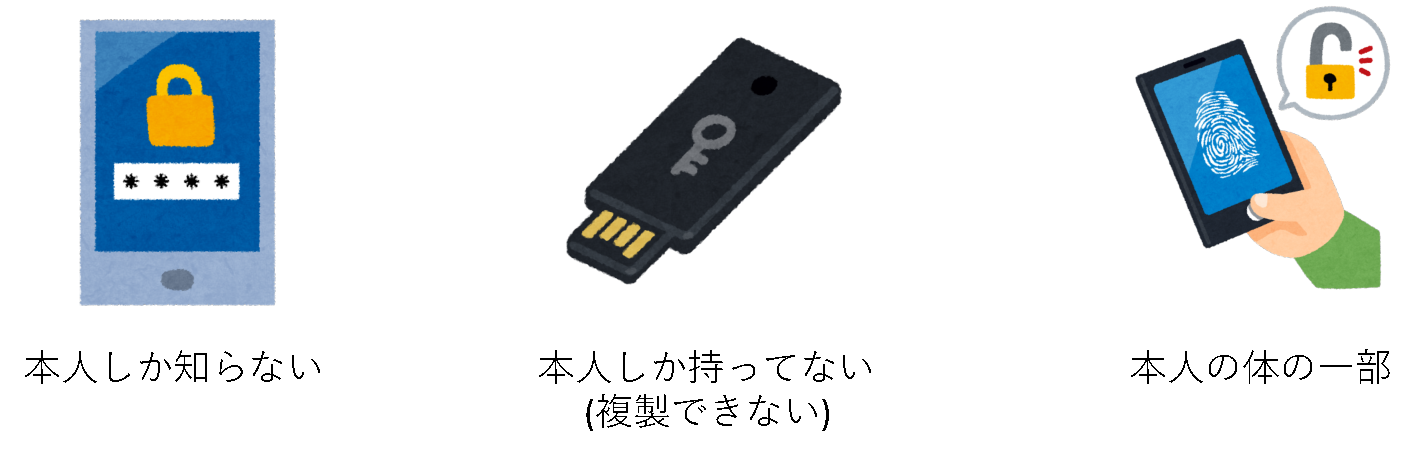
\includegraphics[width=0.7\linewidth]{Figs/auth-three-elements.pdf}
\end{center}

\end{frame}

\begin{frame}{オンラインサービスでのパスワード認証}
\begin{itemize}
\item サービスの利用者の識別子 (ID) と対応するパスワードをサービス事業者に登録、サービス利用時に利用者が自分のIDとパスワードを入力する。
\item パスワードは個人の記憶にのみ存在するため、\alert{パスワードを知っている人はそのサービスに登録してる本人と同一人物}と考えることができる。
\end{itemize}

\begin{center}
おそらく、誰にとっても最も馴染み深い認証方式! 
\end{center}

\end{frame}

\begin{frame}
\begin{figure}
\centering
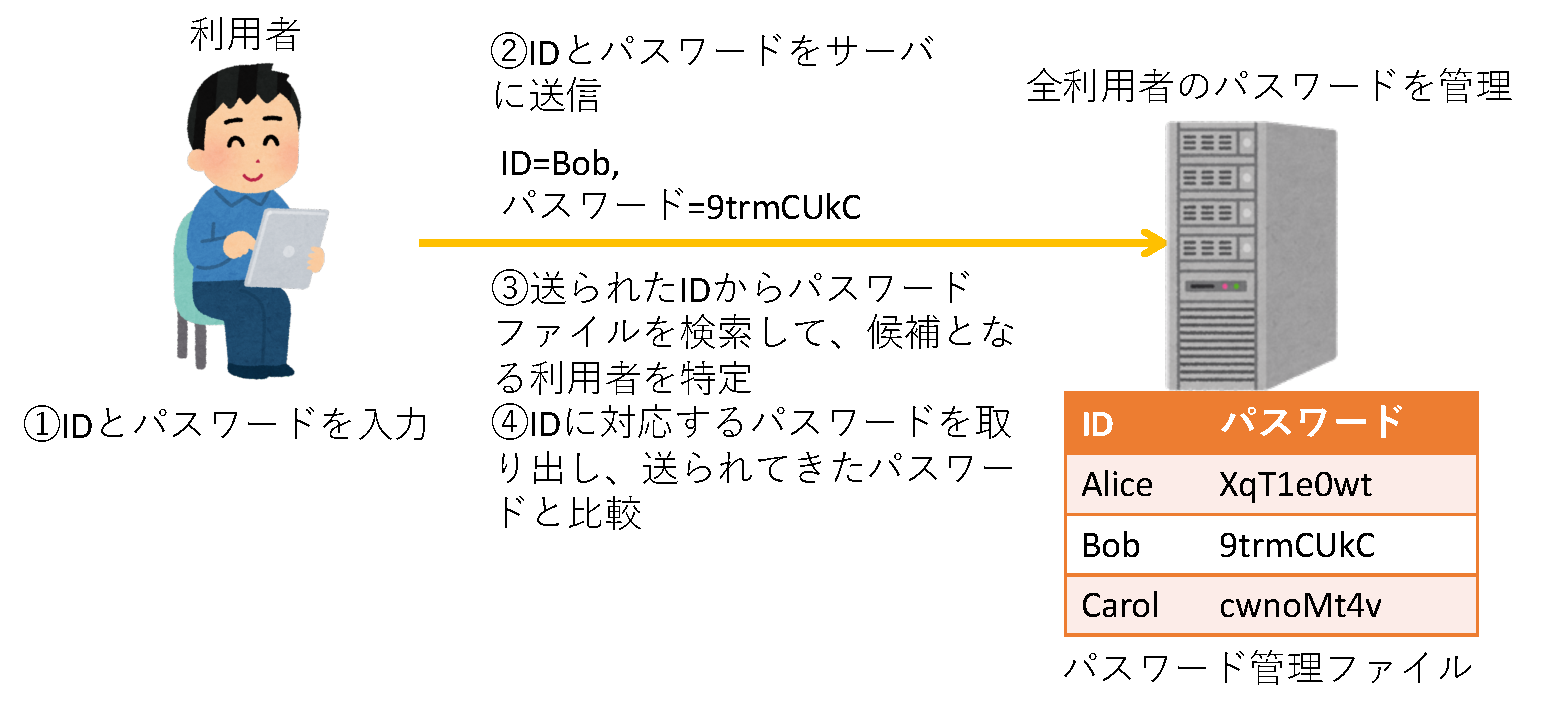
\includegraphics[width=\linewidth]{Figs/password-auth.pdf}\\
\caption{オンラインでの単純なパスワード認証}
\end{figure}
\end{frame}


\begin{frame}{オンラインでのパスワード認証の問題}
英数字・記号を組み合わせたパスワード:
\begin{itemize}
 \item 攻撃者にとって比較的\textbf{予測しやすい}\footnote[frame]{\scriptsize しかもオンラインだと予測→認証トライを繰り返せる}
 \item 「強い」パスワードを使わせるには\textbf{ユーザ教育が必要}\footnote[frame]{\scriptsize 教育なしだと覚え易く「弱い」ものを利用しがち}
 \item \textbf{覚えられない}
 \item etc...
\end{itemize}

\vspace{-5ex}
\begin{center}
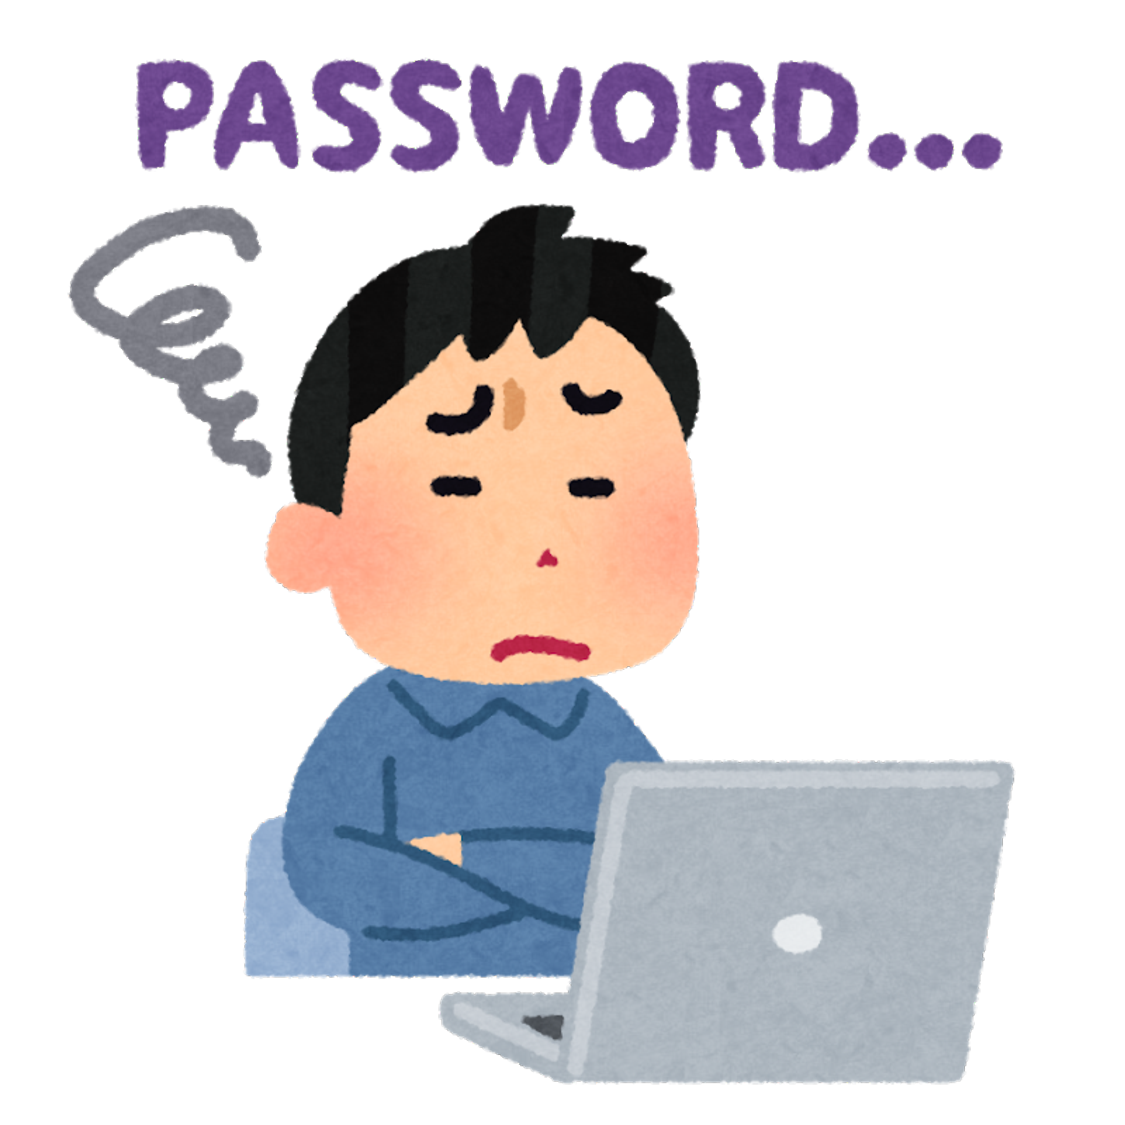
\includegraphics[width=0.2\linewidth]{Figs/password-forget.pdf}
\end{center}
\vspace{-2ex}

\structure{予測できず、誰が使っても強力で、確実に認証できる方法}が必要\\
$\Rightarrow$ \alert{ハードウェアセキュリティキーを使った認証}が人気に\\
$\Rightarrow$ \textbf{FIDOはそのような手法の\ul{標準化された方式}}

\end{frame}

\begin{frame}{FIDO}

\begin{block}{\small FIDO (Fast IDentity Online)}
業界団体FIDO Alliance\footnote[frame]{\scriptsize \url{https://fidoalliance.org}}の策定する、\alert{ハードウェアセキュリティキー+生体認証\footnote[frame]{\scriptsize すなわち、「所有物」と「生体」の二要素を同時に使った認証が可能。}と公開鍵暗号方式をベースとしたオンラインでの本人認証技術}。
\end{block}

現在はFIDO2 (v2.0) が最新の規格。以降、FIDO2の内容について触れていく。

\vspace{2ex}

厳密には、\structure{FIDO2はパスワードレス認証をサポートしつつも、パスワード+デバイス・生体認証の多要素での認証もサポートする}。

\end{frame}

\begin{frame}{FIDO認証概略}
FIDO認証の特徴:
\begin{itemize}
 \item 公開鍵暗号を利用した、オンラインでの認証方式の提供
 \item 認証器によるローカルでの本人認証
 \item 認証器内部に閉じた署名生成\\ $\Rightarrow$\alert{秘密鍵・パスワード等の秘密情報は外部に出ない}
\end{itemize}
\begin{figure}
\begin{center}
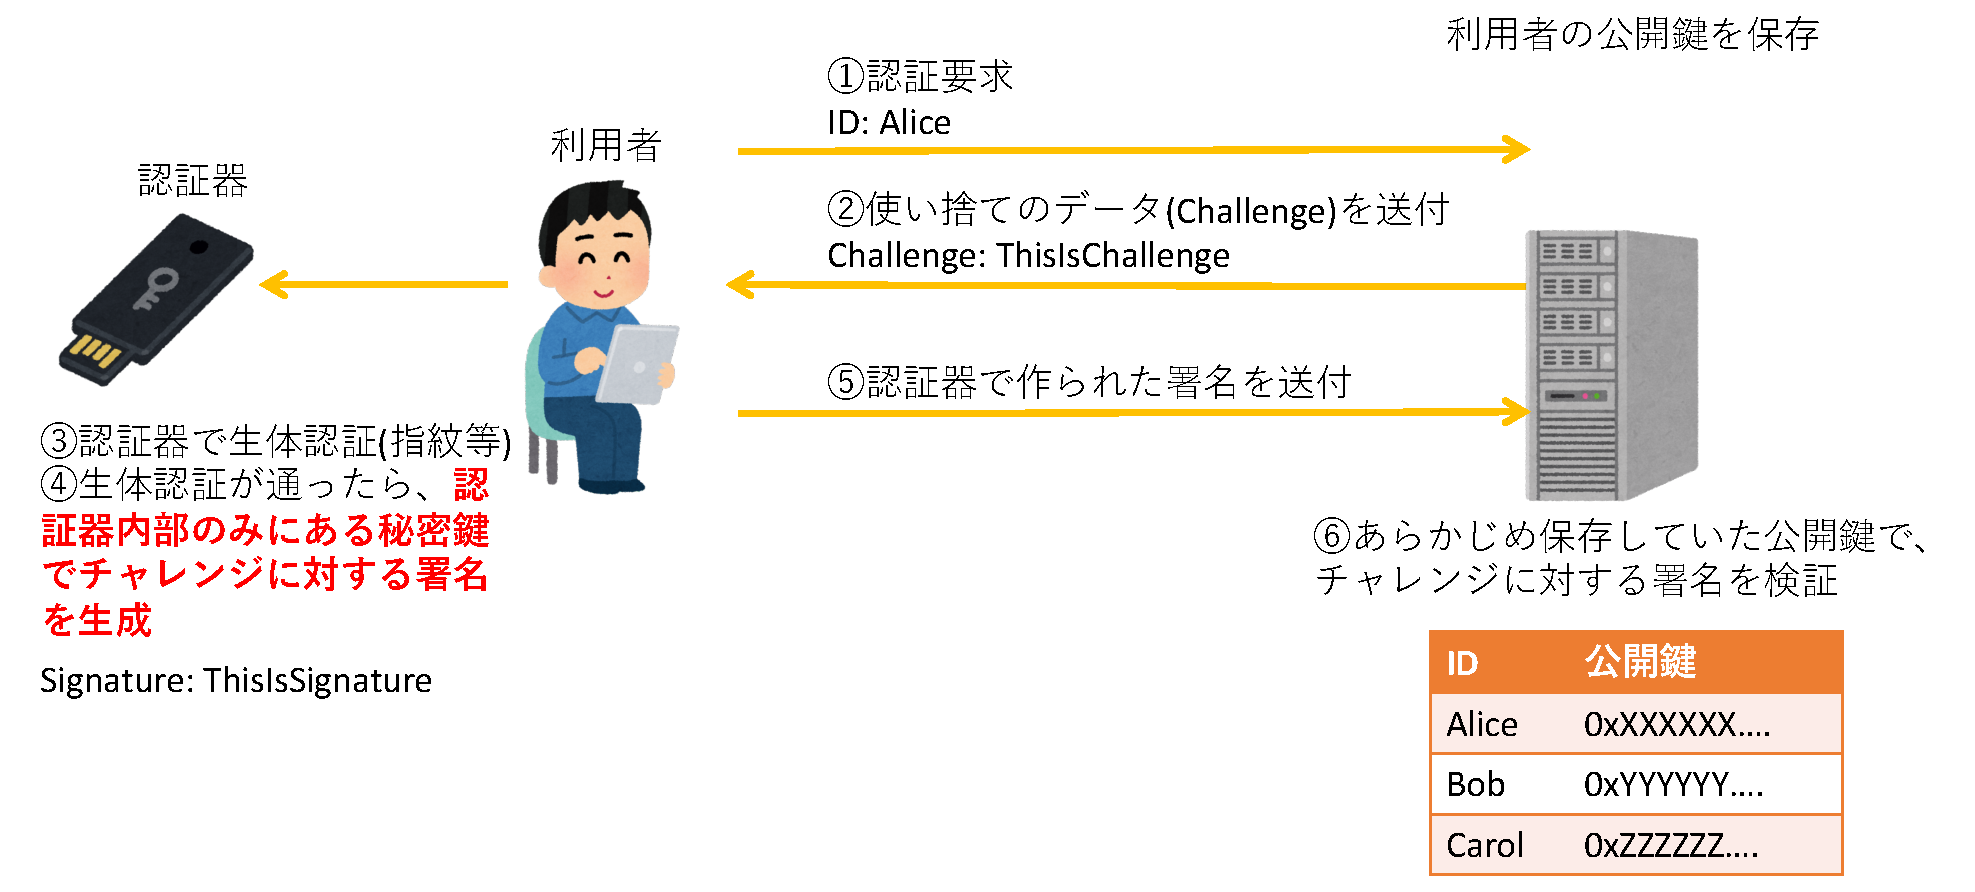
\includegraphics[width=0.9\linewidth]{Figs/FIDO2-auth.pdf}
\caption{FIDO認証概略}
\end{center}
\end{figure}
\end{frame}

\begin{frame}{FIDO2の要素}
FIDO2は、\alert{WebAuthn (Web Authentication)\footnote[frame]{\tiny Spec: \url{https://www.w3.org/TR/webauthn-1/}}と、CTAP (Client-to-Authenticator Protocol)\footnote[frame]{\tiny Spec: \url{https://fidoalliance.org/specs/fido2/fido-client-to-authenticator-protocol-v2.1-rd-20191217.html}}の2つの要素で構成}される。

\begin{itemize}
 \item \textbf{WebAuthn}: 内部/外部認証器をCallするWebAPIと、WebApp・サーバ間のデータフローを規定。
 \item \textbf{CTAP}: 外部認証器をCallするAPIと、クライアント/プラットフォームと認証器の通信プロトコルを規定。
\end{itemize}
\end{frame}

\begin{frame}
図で見るとCTAP・WebAuthnは以下のような役割分担。
\begin{center}
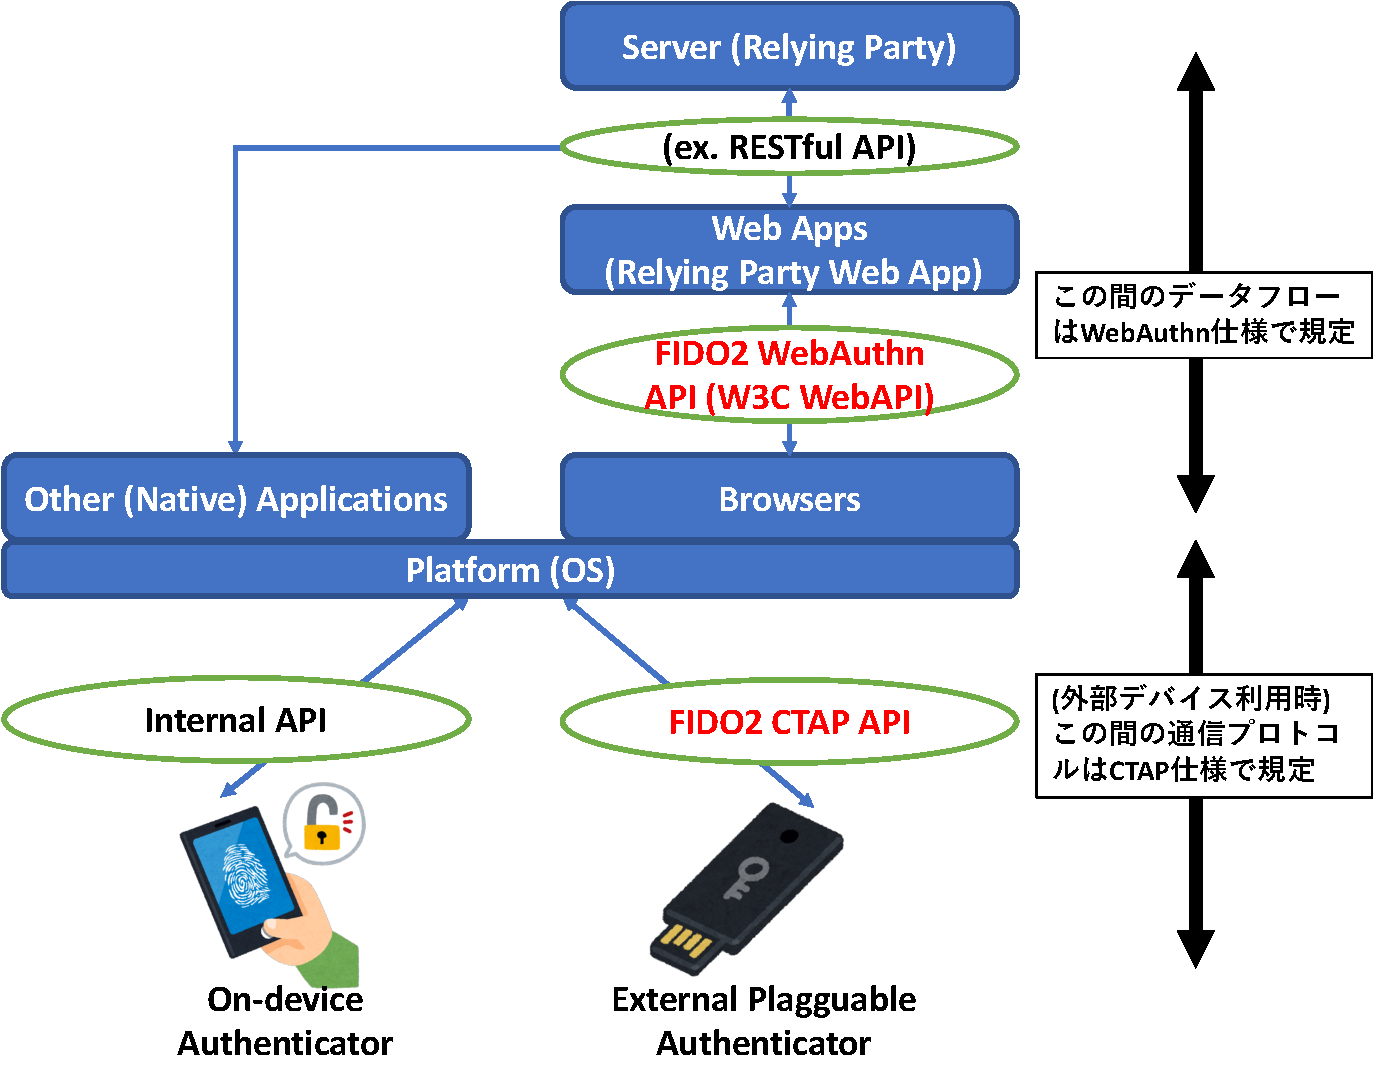
\includegraphics[width=0.8\linewidth]{Figs/FIDO2-spec-structure.pdf}
\end{center}
\end{frame}

\begin{frame}
\begin{block}{\small FIDO2 CTAP\footnote[frame]{\tiny \url{https://fidoalliance.org/specs/fido-v2.0-ps-20190130/fido-client-to-authenticator-protocol-v2.0-ps-20190130.html}}}
USB/BLE/NFC等で接続されたHWセキュリティキーなどの\alert{外部認証器と、クライアントアプリ(ブラウザ等)およびプラットフォーム(OS)との間の通信プロトコル}を規定。以下の要素で構成。
\begin{itemize}
\item USB/BLE/NFCなど物理層の種別に応じた、通信確立のためのプロトコル
\item 認証器での処理をCallするAPI
\begin{itemize}
\item 外部認証器の情報取得
\item PINによるローカルでのユーザ認証\footnote[frame]{\tiny 指紋認証やジェスチャーなどは認証器のみで完結するのでAPIは用意されない。署名生成などのときに認証器内での認証を要求するフラグを立てる。}
\item 認証器組込の秘密鍵での、ユーザ秘密鍵・証明書生成
\item ユーザ秘密鍵による署名の生成、など
\end{itemize}
\end{itemize}
\end{block}
ブラウザ・OS(のドライバ)は上記を実装した上で、より上位のWebAuthnのプロトコルをサポート。
\end{frame}


\begin{frame}
\begin{block}{\small FIDO2 WebAuthn\footnote[frame]{\tiny https://www.w3.org/TR/webauthn-1/}}
\alert{Webブラウザをプラットフォームとし、内部/外部認証器によって生成される署名を用いた、オンラインサーバでのユーザ認証のプロトコル}を規定。
より具体的には、以下を規定する。
\begin{itemize}
 \item 認証器でのユーザの公開鍵証明書の生成、サーバへの登録プロトコル
 \item 認証器での署名生成、サーバでの認証プロトコル
 \item 認証器とやりとりするためブラウザが具備すべきWeb API\footnote[frame]{\tiny JavaScriptでCallされるAPI。ブラウザの内部でさらに認証器のAPI (CTAPや内部API) をCallする。}。大雑把に以下の2種類。
\begin{itemize}
 \item ユーザの公開鍵証明書の生成 (Credential Creation)
 \item ユーザ秘密鍵による署名の生成 (Assertion Generation)
\end{itemize}
\end{itemize}
\end{block}
認証器とのやり取りはブラウザ/プラットフォームがサポート。\\
$\Rightarrow$ 基本的にWeb Appの観点からは、WebAuthnのみを意識する。
\end{frame}


\begin{frame}
\begin{exampleblock}{\small 補足: FIDO1}
\small
FIDO1 (v1.x) は、以下の2つの要素で構成されている。
\begin{itemize}
 \item UAF (Universal Authentication Framework): 生体認証機能を持つFIDO対応端末 (スマートフォン等) で\structure{パスワードレス認証}を行う機構。USB接続などの外部HWセキュリティキーは利用できない。
 \item U2F (Universal 2nd Factor)\footnote[frame]{\scriptsize U2FはFIDO2規格ではCTAP1と改称。FIDO2で追加された仕様はCTAP2と呼ばれる。}: ID・パスワード認証に加えた\structure{2要素認証}を行うのに、外部HWセキュリティキーを利用可能とする機構。
\end{itemize}
FIDO2は、UAFとU2Fを統合し、さらに外部HWキーを用いてもパスワードレス認証可能な、より利便性の高い規格と見做せる。
\end{exampleblock}
 
\end{frame}


\begin{frame}
\frametitle{FIDO2対応の認証器}
USB/NFC/BLE等対応の外部認証器 (External Authenticator)、端末付属の認証器 (On-device/Internal Authenticator) 共々、様々な対応デバイスがリリースされつつある。
\begin{tabular}{ccc}
\begin{minipage}[t]{0.3\linewidth}
\footnotesize
\centering
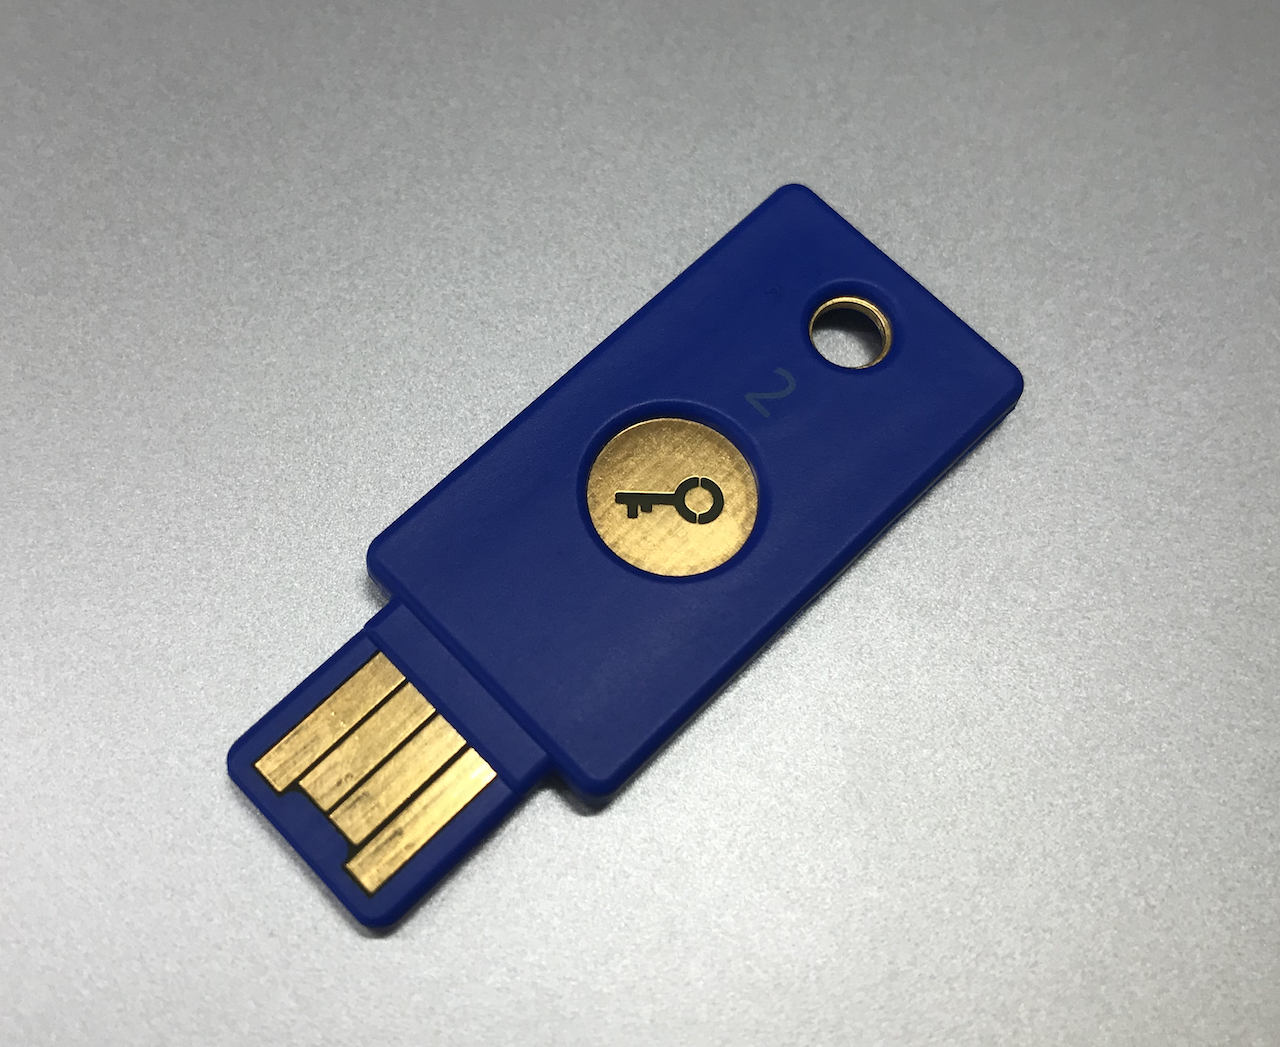
\includegraphics[width=\linewidth]{Figs/security-key-by-yubico.png}\\
\textbf{Security Key by Yubico}\\
FIDO2専用\footnote[frame]{\scriptsize FIDO2 CTAP1=FIDO1 U2Fには対応。}
\end{minipage}
& 
\begin{minipage}[t]{0.3\linewidth}
\footnotesize
\centering
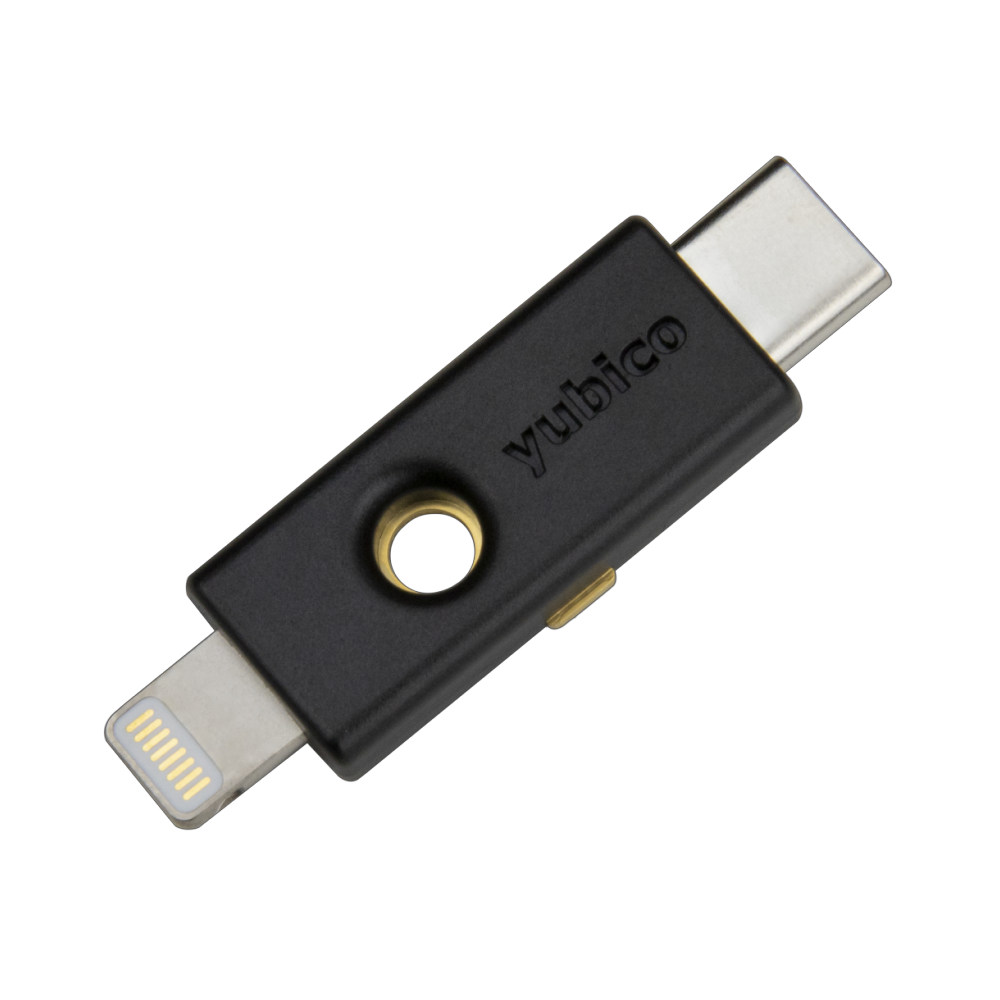
\includegraphics[width=\linewidth]{Figs/yubikey-5ci.png}\\
\textbf{YubiKey 5Ci}\\
FIDO2+OpenPGP+etc...
\end{minipage}
&
\begin{minipage}[t]{0.3\linewidth}
\footnotesize
\centering
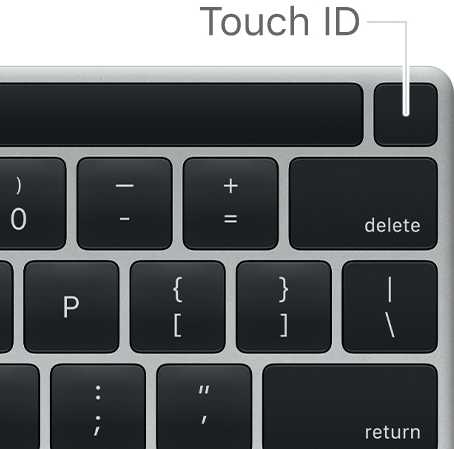
\includegraphics[width=\linewidth]{Figs/macbookpro-touchid.png}\\
\textbf{MacbookPro TouchID}\\
FIDO2認証可能\footnote[frame]{\scriptsize ブラウザ等がTouchID APIをCallできればFIDO2のOn-device Authenticatorとして動作。Chrome等は対応済。}
\end{minipage}
\end{tabular}
\end{frame}


\begin{frame}{FIDO2標準化状況}

FIDOは業界団体の策定した規格ではあるが、

\begin{itemize}
 \item \textbf{FIDO2 CTAP}: ITU-Tで勧告として国際標準化\footnote[frame]{\scriptsize \url{https://fidoalliance.org/fido-alliance-specifications-now-adopted-as-itu-international-standards/}}
 \item \textbf{FIDO2 WebAuthn}: W3Cで勧告として国際標準化\footnote[frame]{\scriptsize \url{https://www.w3.org/2019/03/pressrelease-webauthn-rec.html.ja}}
\end{itemize}

と、認証器とプラットフォーム/ブラウザ間の通信プロトコル、サーバ・ブラウザ間の認証プロトコルの両者共に国際標準として策定済。

\end{frame}

\begin{frame}
この後、FIDO2 WebAuthnの内容に実際に触れ、最新の認証技術について理解を深めてみよう。\footnote[frame]{\scriptsize 今回はWeb技術から学ぶセキュリティに注力するため、ローレイヤのFIDO2 CTAPについては別の機会で。}
\end{frame}

%%%%%%%%%%%%%%%%%%%%%%%%%%%%%%%%%%%%%%%%%%%%%%%%%%%%%%%%%%%%%%%%%%%%%%%%%%%%%%%%%%%%%%%%%%%%%%%%%%%
\section{実験環境の準備}
\begin{frame}
\centering
{\Large 実験環境の準備}
\end{frame}

\begin{frame}{準備}
説明を聞きつつ手を動かすため、まず環境準備。

\vspace{2ex}

今回は以下の2つをWebAuthnのAPIをCallしながら実験してみる。
\begin{itemize}
\item 認証器を使って「ユーザ登録」\\
$\Rightarrow$ 認証器からのメッセージを解してみて\structure{実際に証明書および生の公開鍵を取り出してみる}。
\item 認証器を使って「ユーザ認証」\\
$\Rightarrow$ 署名を解してみて、登録時に取り出した公開鍵で\structure{署名が通ることを確認してみる}。
\end{itemize}
$\Rightarrow$ この2つが\alert{FIDO2 WebAuthnのパスワードレス認証の基礎}。
\end{frame}

\begin{frame}
\frametitle{環境}

以下の環境が前提:
\begin{itemize}
 \item Node.js LTS ($\ge$ 12)がインストール済でyarnが使える\footnote[frame]{インストールコマンド: \texttt{npm i -g yarn}}
 \item ブラウザとして、Google Chrome (系ブラウザ)、もしくはFirefoxがインストール済み
 \item Visual Studio Code や WebStorm などの統合開発環境がセットアップ済みだとなお良い
\end{itemize}
\end{frame}

\begin{frame}
\frametitle{JavaScriptプロジェクトの準備}
\begin{enumerate}
\item \alert{プロジェクトのGitHubリポジトリをClone}\\
\begin{exampleblock}{}
\footnotesize
\$ \texttt{git clone https://github.com/junkurihara/class-fido2\_webauthn.git}\\
\$ \texttt{cd sample}
\end{exampleblock}
\item 依存パッケージのインストール
\begin{exampleblock}{}
\$ \texttt{yarn install}
\end{exampleblock}
\item ライブラリのビルド
\begin{exampleblock}{}
\$ \texttt{yarn build}
\end{exampleblock}
\end{enumerate}
\end{frame}

\begin{frame}{認証器の準備}
実験の前に認証器をセットアップしておく。例えば「Security Key by Yubico」の場合は、「YubiKey Manager」をインストールし、PINを設定。\footnote[frame]{\scriptsize 「PIN+認証器へのタッチ」が生体認証という扱い。PIN設定はなくても動作するが、タッチだけで生体認証したことになってしまう。PINではなく指紋認証を使うような認証器では、指紋登録が前もって必要。}
\begin{figure}
\begin{center}
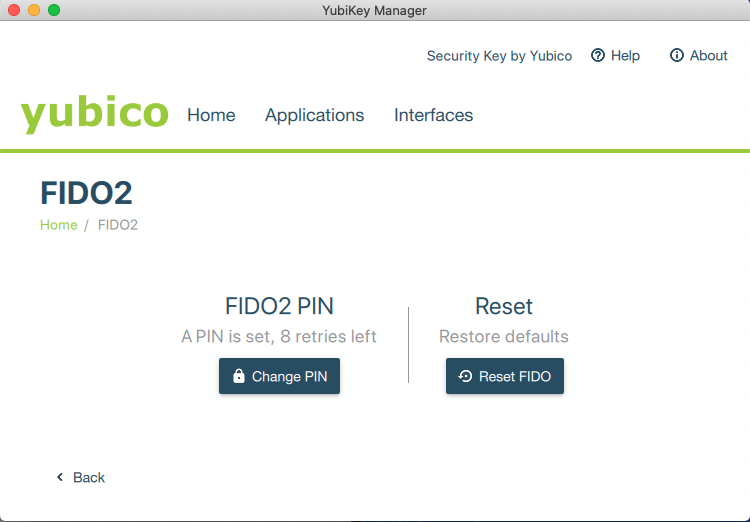
\includegraphics[width=0.4\linewidth]{Figs/yubikey-manager.png}
\end{center}
\caption{YubiKey Manager (Mac)}
\end{figure}
\end{frame}


%%%%%%%%%%%%%%%%%%%%%%%%%%%%%%%%%%%%%%%%%%%%%%%%%%%%%%%%%%%%%%%%%%%%%%%%%%%%%%%%%%%%%%%%%%%%%%%%%%%
\section{FIDO2 WebAuthn}
\begin{frame}
\centering
{\huge FIDO2 WebAuthn}
\end{frame}

\subsection{WebAuthn 事始め}

\begin{frame}
\centering
{\Large FIDO2 WebAuthn 事始め}
\end{frame}

\begin{frame}{FIDO2 WebAuthnのフローの参加エンティティ}
WebAuthnの動作フローでは、以下の3つの(抽象化された)参加エンティティが存在。
\begin{enumerate}
 \item \textbf{Relying Party (RP)}: サービス提供者の認証サーバ
 \item \textbf{ブラウザ+RPのWebApp}: ユーザおよび認証器とやり取り
 \item \textbf{Authenticator}: 内部/外部認証器。以下をセキュアに保持。
\begin{itemize}
\item \textbf{\alert{Attestation Key Pair}}: 公開鍵・秘密鍵ペア
\item \textbf{\alert{Attestation Certificate}}: 上記の公開鍵に対し、FIDO2で承認された製造元が署名した証明書
\end{itemize}
\end{enumerate}
\end{frame}
\begin{frame}
\begin{center}
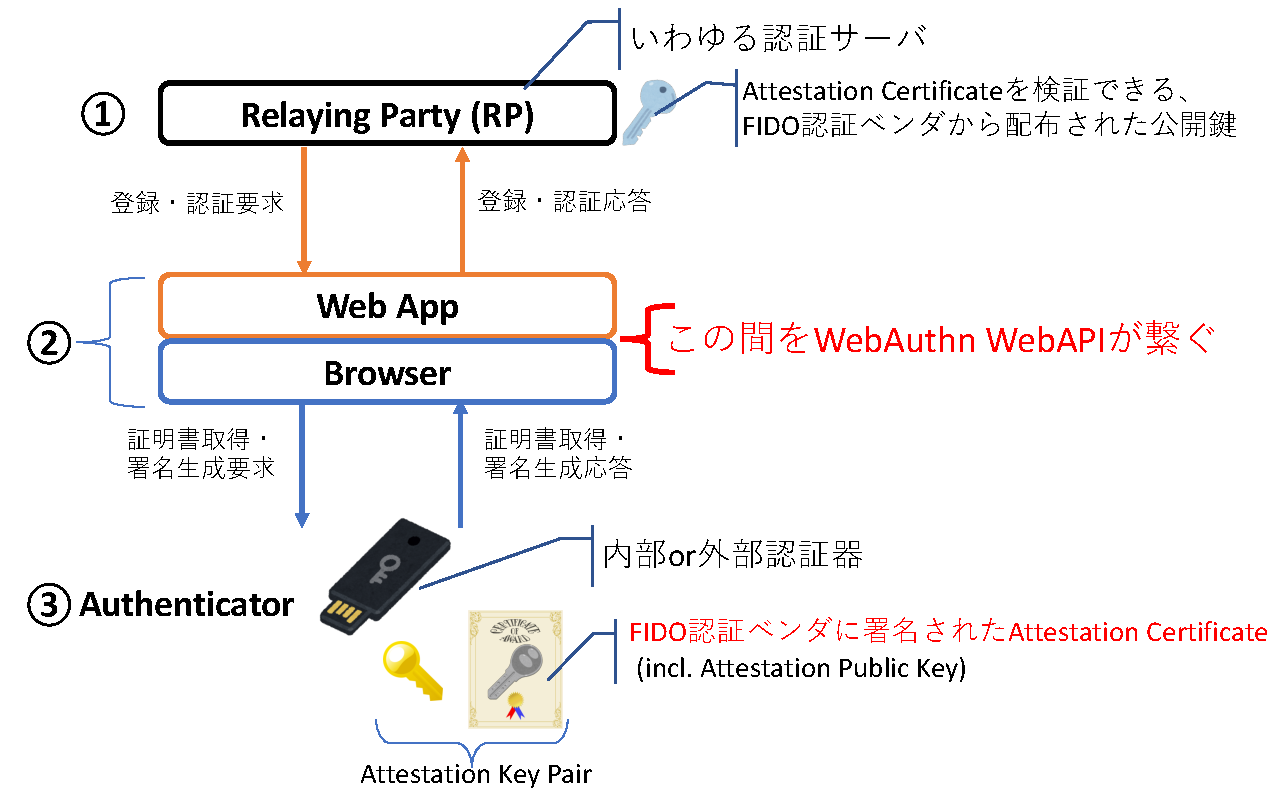
\includegraphics[width=0.9\linewidth]{Figs/webauthn-entities.pdf}
\end{center}
WebAPIとして用意されるWebAuthn APIは、ブラウザ経由でWebAppが認証器とやりとりする役割を担う。
\end{frame}

\begin{frame}{FIDO2 WebAuthnの2つのフロー}
FIDO2 WebAuthnは、2つの動作フローを規定する。
\begin{itemize}
 \item \alert{\textbf{ユーザ登録フロー}}: 認証器を使って、Relying PartyにユーザのIDや認証情報=公開鍵\footnote[frame]{\scriptsize Credential Public Key/Certificateのこと}を登録する処理
 \item \alert{\textbf{ユーザ認証フロー}}: 認証器を使って、Relying Partyに事前に認証情報を登録したユーザ自身であることを証明する処理。
\end{itemize}

\vspace{2ex}

以降、この2つのフローの中身を見ていくが、その前にFIDO2 WebAuthnにおいて\textbf{登録・認証の安全性を担保するAttestation}という概念について解説しよう。
\end{frame}

\begin{frame}{FIDO2におけるAttestation}
FIDO2では、「Attestation」という重要な概念が存在する。

\begin{block}{\small FIDO2におけるAttestation}
主として、「新しく生成・登録するユーザの公開鍵が、\alert{正しくFIDO2認定を受けている認証器で生成された公開鍵であることを保証する機構}」という意味。すなわち、\textbf{出生証明}。
\end{block}
\begin{center}
\begin{tabular}{ll}
\begin{minipage}[c]{0.8\linewidth}
Relying Partyは、出生証明を確認してユーザを登録。\\
$\Rightarrow$ 偽造認証器を摑まされたユーザの登録を弾ける。\\
$\Rightarrow$ \textbf{認証器に基づくFIDO2認証の安全性は維持}。
\end{minipage}
 &
\begin{minipage}[c]{0.15\linewidth}
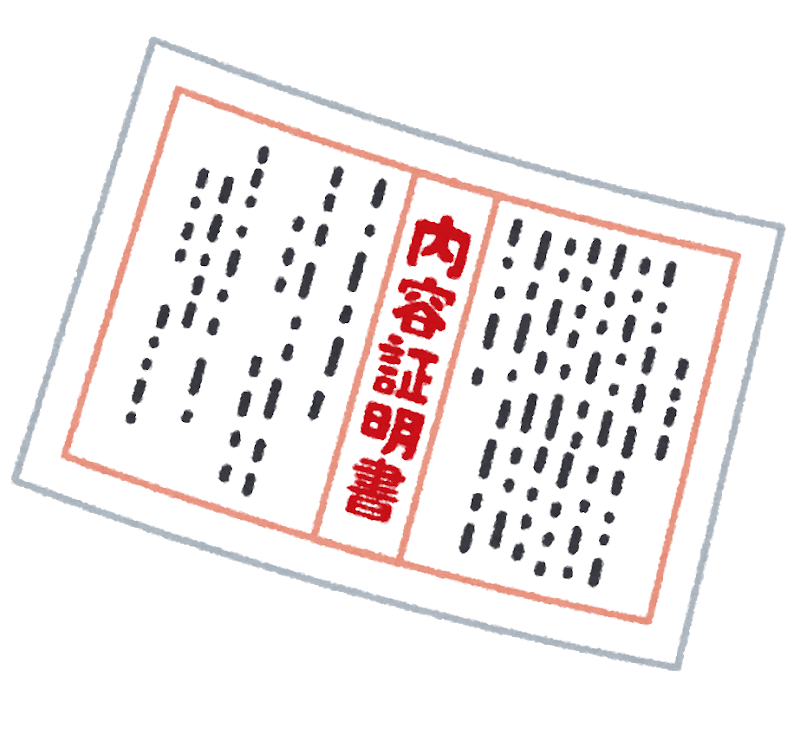
\includegraphics[width=\linewidth]{Figs/naiyo-shomei.png} 
\end{minipage}
\end{tabular}
\end{center}

※認証器で生成するユーザの鍵ペアを\alert{Credential Key Pair}、Attestされたその公開鍵を\alert{Attested Credential Public Key}と呼ぶ。
\end{frame}

\begin{frame}
\small 
Attestationの流れ。Attestationは2段階の証明で成立:
\begin{center}
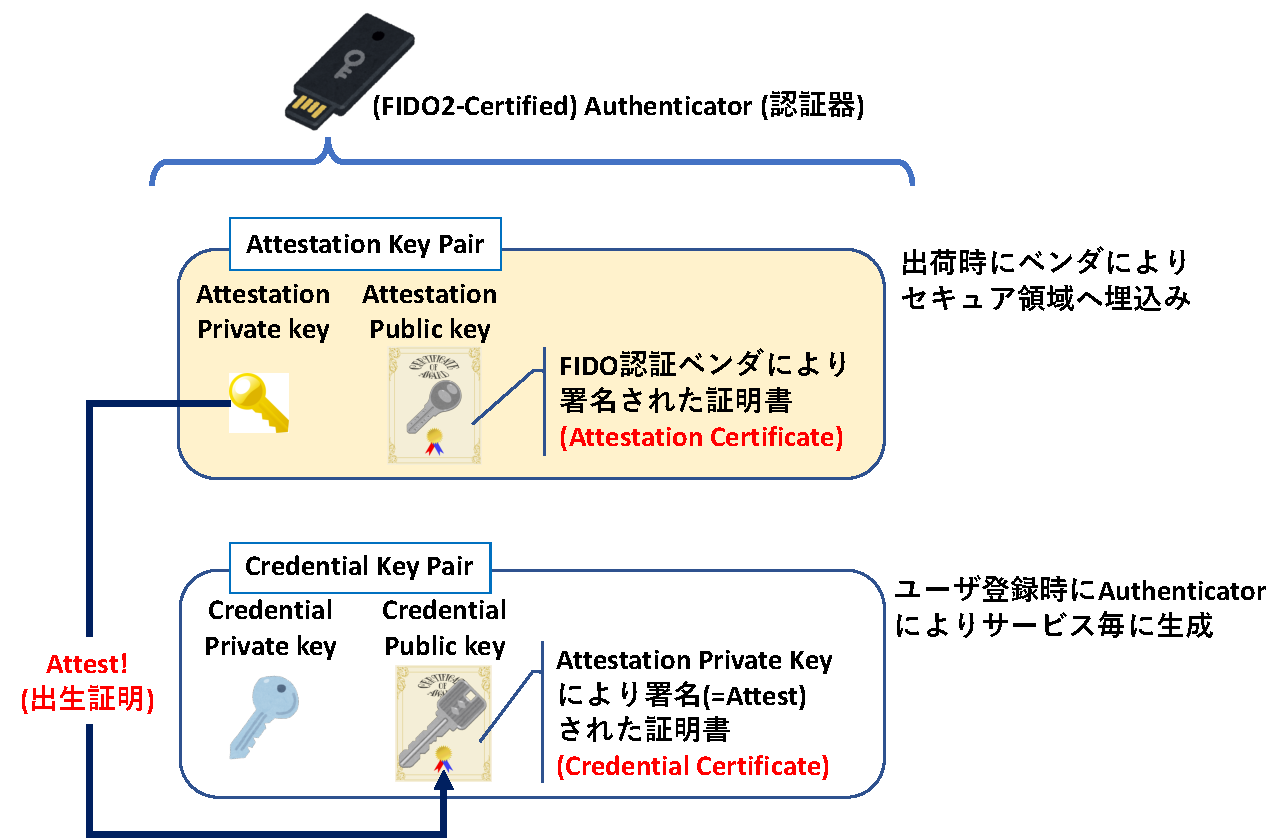
\includegraphics[width=0.7\linewidth]{Figs/webauthn-attestation.pdf}
\end{center}

ユーザ登録時にユーザ公開鍵(Credential Public Key)を出生証明して登録\\
$\Rightarrow$ Attested Credential Public Keyの署名をAttestation Certificateで検証\\
$\Rightarrow$ Attestation CertificateをFIDO認証ベンダの公開鍵\footnote[frame]{\scriptsize ルート証明書}で検証
\end{frame}

\begin{frame}
\small
\begin{exampleblock}{\small 補足: Attestationの種類}
\footnotesize
\begin{itemize}
\setlength{\itemsep}{0ex}
 \item \textbf{Basic}: ベンダが認証器モデルごとに特有のAttestation Key Pairを埋込む。同じモデルの認証器では同じ鍵ペアでも良い。
 \item \textbf{Self}: Attestation Private Key = Credential Private Keyとして、自分の秘密鍵で署名して自己Attestする。
 \item \textbf{AttCA}\footnote[frame]{\scriptsize Attestation Certificate Authority}: Attestation Certificateを動的に生成する手法。外部に信頼できる第三者の認証局を設け、認証器がAttestation (Identity) Key Pairを生成して、認証局へその公開鍵への署名を依頼。
 \item \textbf{ECDAA}\footnote[frame]{\scriptsize Elliptic Curve based Direct Anonymous Attestation; アルゴリズム仕様は現状ドラフト。}: 楕円曲線上の匿名認証 (Direct Anonymous Attestation; DAA) を利用して、認証器の情報を与えることなく出生証明を実現。
 \item \textbf{None}: Attestationなし。
\end{itemize}
\end{exampleblock}
\textbf{この資料ではBasic前提}。

BasicでもHW構造的に\alert{秘密鍵は認証器から取出せない}。
AttCAでは、認証器のTPMに埋め込まれた鍵を、証明書生成ではなく認証局との暗号通信用に用いる。
\end{frame}

\begin{frame}{この後やってみること}
\small
この後は、
\begin{itemize}
 \item ユーザ登録フロー 
 \item ユーザ認証フロー
\end{itemize}
の両者において、\ul{localhostでRPを模擬}\footnote[frame]{\scriptsize ブラウザ・RPとのやりとりは標準がないことと、処理フロー・データフローを理解することに重点をおくため。しかしPython Flask等でREST APIでやりとりするサーバは簡単に実装可能。}しつつ、認証器・ブラウザ間でやりとりされるデータと、認証器内部での処理をコードを見ながら確認・解説していく。
\end{frame}

\begin{frame}[fragile]
以下のコマンドをとりあえず叩いてみると、ブラウザ (Google Chrome) が立ち上がって認証器の挿入を求められることが確認できる。

\begin{exampleblock}{\footnotesize ユーザ登録→ユーザ認証の一連のテストコードを実行}
\footnotesize
\begin{verbatim}
$ yarn test // sampleディレクトリで実行
\end{verbatim}
\end{exampleblock}

この時に行われている動作を解説する。
\end{frame}


\subsection{WebAuthn ユーザ登録フロー}

\begin{frame}
\centering
{\Large FIDO2 WebAuthn ユーザ登録フロー}
\end{frame}


\begin{frame}{WebAuthn ユーザ登録フロー}
以下のような流れでWebAuthnの認証のための登録を行う。
\begin{center}
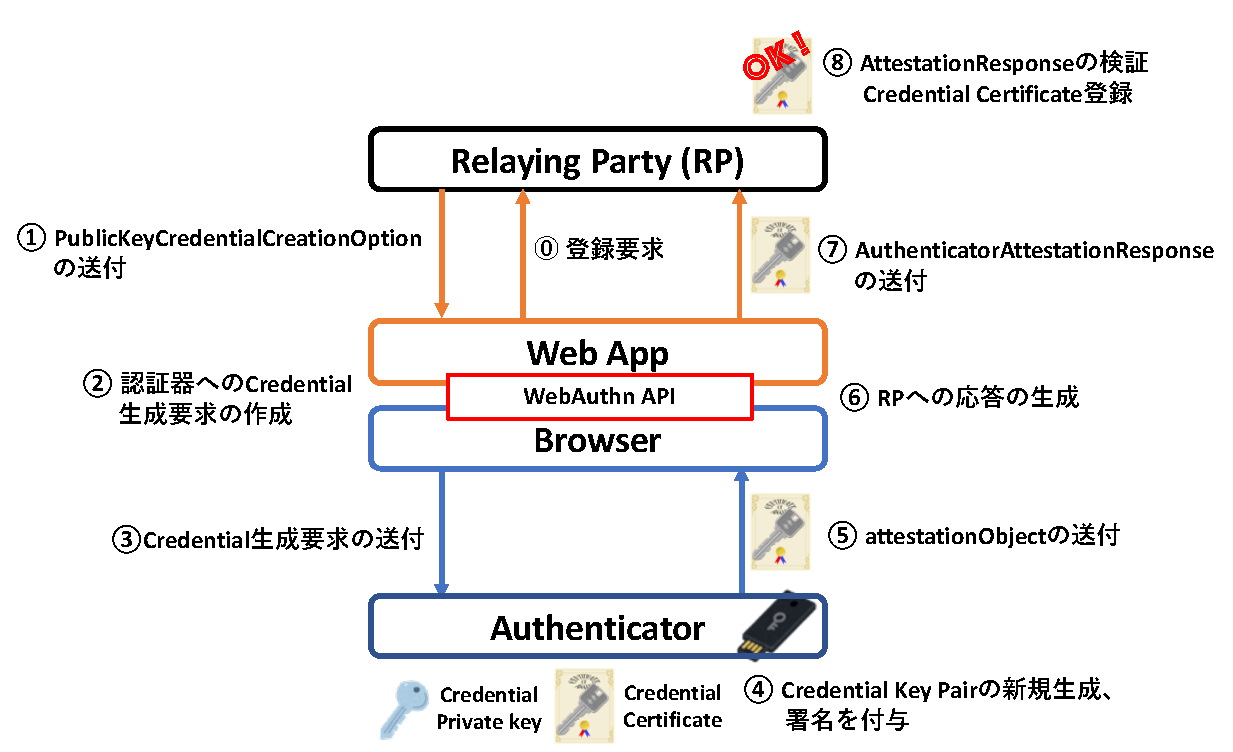
\includegraphics[width=0.9\linewidth]{Figs/webauthn-registration0.pdf}
\end{center}
単純に言うと、\textbf{認証器でCredential Public Keyを生成、その出生証明をRPで確認・登録}という処理。

\end{frame}

\begin{frame}
このユーザ登録の各ステップを、実際のデータを確認しながら追っていく。
\end{frame}

\begin{frame}{WebAuthn ユーザ登録: RPへユーザ登録要求}
⓪,① ユーザ登録のためCredential生成パラメタをRPから取得。
\begin{center}
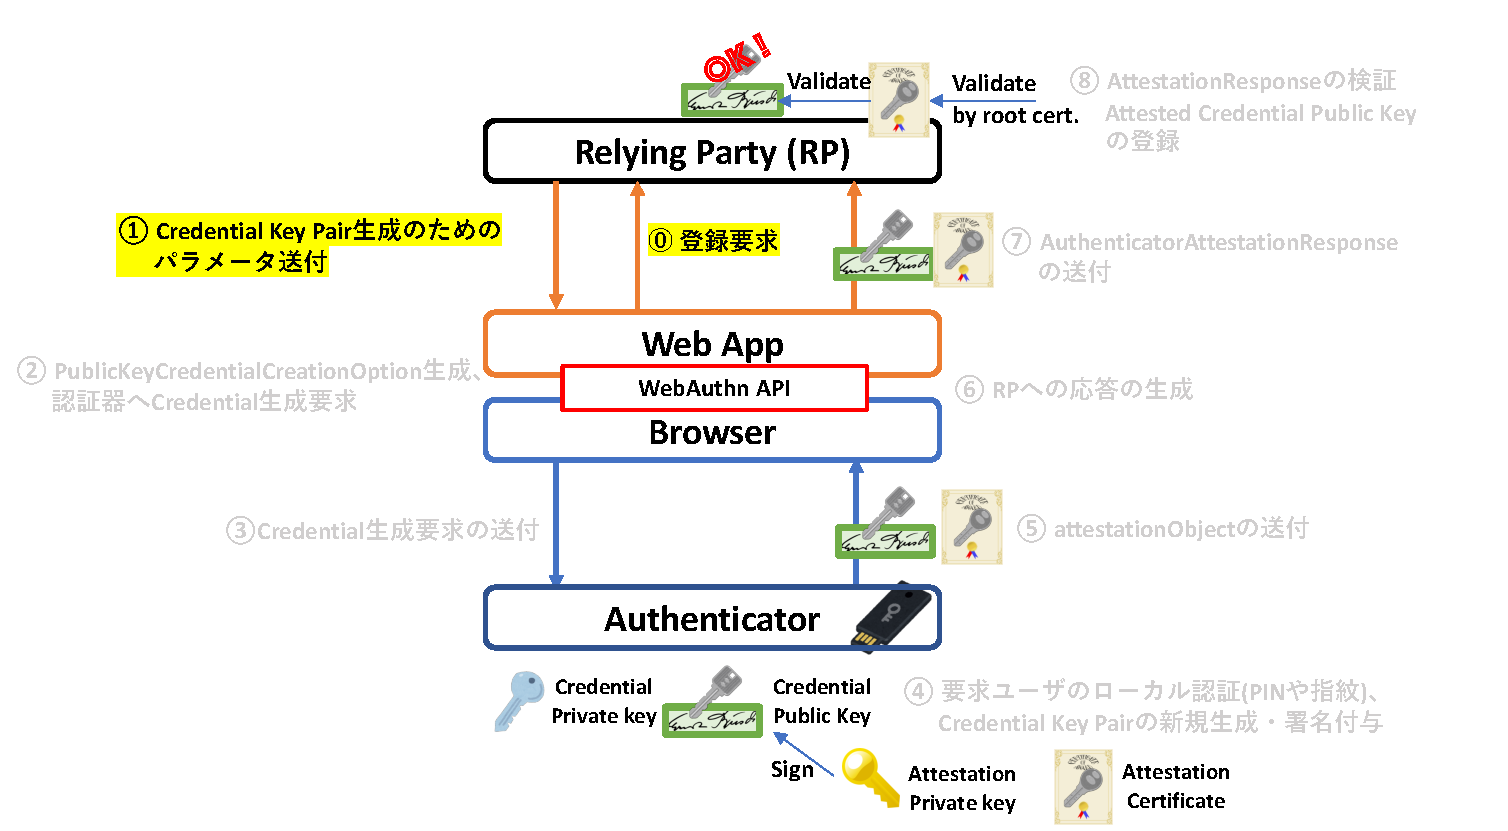
\includegraphics[width=0.9\linewidth]{Figs/webauthn-registration1.pdf}
\end{center}
\textbf{WebAppとRP間の要求・応答フォーマットは規定されていない。}\\
$\Rightarrow$ RP側の (REST) APIは実装者に任せられている。
\end{frame}

\begin{frame}
WebAppがRPから取得するパラメタは以下の通り。\footnote[frame]{\scriptsize UserInfo, RP InfoはWebAppすなわちユーザが自分で定めることも(一応)できる。}
\begin{itemize}
 \item \textbf{Challenge}: \alert{暗号学的にランダムな使い捨てのbinary string (最低16bytes, 通常32bytes程度)}
 \item \textbf{User Info}: ユーザ情報。ID、メールアドレス、名前。
 \item \textbf{Relying Party Info}: RP(すなわちサービス)の名前、FQDN、サービスアイコンのURL (icoファイル)。
\end{itemize}

\vspace{2ex}
ブラウザは、これらを\texttt{PublicKeyCredentialCreationOptions} Objectにし、WebAuthn API経由で認証器へCredential生成を要求。

\end{frame}

\begin{frame}{WebAuthn ユーザ登録: 認証器へCredential生成要求}
②,③ ブラウザのAPIをCallして認証器へCredential生成を要求。
\begin{center}
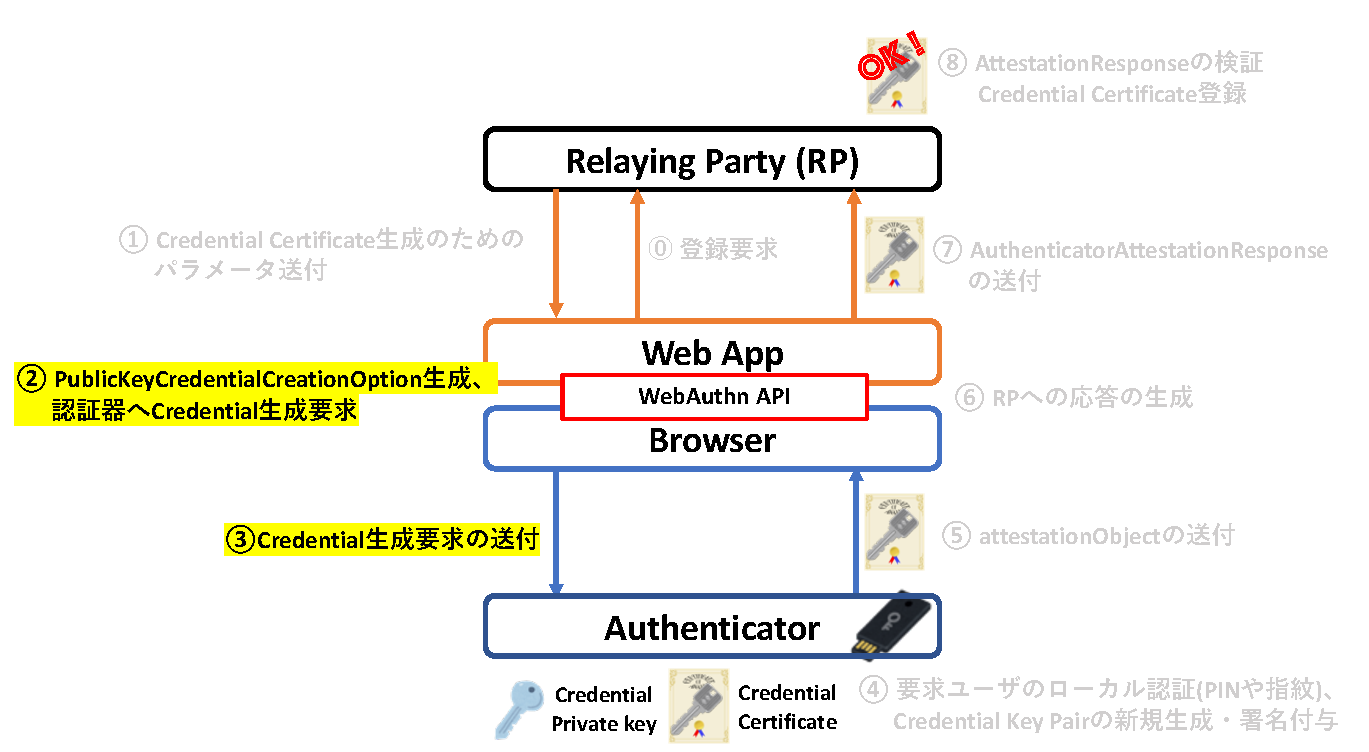
\includegraphics[width=0.9\linewidth]{Figs/webauthn-registration2.pdf}
\end{center}
\texttt{PublicKeyCredentialCreationOptions} Objectをブラウザの\texttt{window.navigator.credential.create()}へ入力。
\end{frame}

\begin{frame}[fragile]
\small
\textbf{②: \texttt{認証器に送るオブジェクトの生成}}

\begin{exampleblock}{\scriptsize \texttt{PublicKeyCredentialCreationOptions}の構造 (\texttt{./test/credential-params.ts)}}
{\tiny
\begin{verbatim}
const createCredentialDefaultArgs: CredentialCreationOptions = {
  publicKey: {
    // Challenge 本当はサーバーで生成した暗号学的に安全な乱数をセット (16bytes以上)
    challenge: new Uint8Array([0x8C, 0x0A, 0x26, 0xFF, 0x22, ...]).buffer,

    // Relying Party Info (a.k.a. - Service)
    rp: {
      id: 'localhost', // テストコードはローカルで走るため
      name: 'Example RP'
    },

    // User Info
    user: {
      id: new Uint8Array(16),
      name: 'john.p.smith@example.com',
      displayName: 'John P. Smith',
    },

    // 利用したいPublic Key Credential Paramsのリスト (認証器は先頭から試行):
    pubKeyCredParams: [{
      type: 'public-key', // As of March 2019, only 'public-key' is accepted.
      alg: -7 // Signature Algorithm (ECDSA with SHA-256)
    }],

    // Attestation Type (optional, defaultは'none' (RPによるattestation検証なし))
    attestation: 'direct', // 'direct'は認証器の生成したAttestationを直接RPに送るタイプ

    // Time Out (optional, in msec)
    timeout: 60000, // 認証器からの応答をブラウザはどれくらい待つか。
  }
};
\end{verbatim}
}
\end{exampleblock}
\end{frame}

\begin{frame}[fragile]
\small
\textbf{③: \texttt{認証器へオブジェクト送付}}\\[2ex]

\texttt{PublicKeyCredentialCreationOptions} Objectを使ってブラウザのWebAuthn APIを以下のようにCallすると、\alert{認証器の挿入・接続要求、PIN入力要求がブラウザ通知}される。

\begin{exampleblock}{\scriptsize \texttt{window.navigator.credential.create()}のCall (\texttt{./test/test.spec.ts})}
{\scriptsize
\begin{verbatim}
const cred: Credential|null
  = await window.navigator.credentials.create(createCredentialDefaultArgs);
\end{verbatim}
}
\end{exampleblock}

\vspace{2ex}

\begin{tabular}{ccc}
\begin{minipage}{0.4\linewidth}
 \centering
 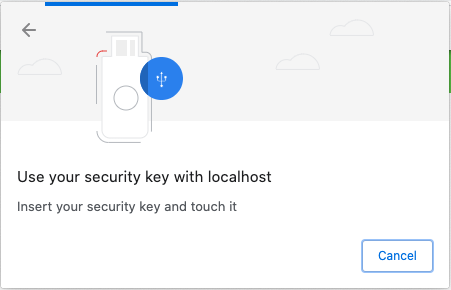
\includegraphics[width=\linewidth]{Figs/webauthn-registration-dialog1.png}\\
 {\footnotesize 認証器挿入・接続要求}
\end{minipage}
 &
$\Rightarrow$
&
\begin{minipage}{0.4\linewidth}
 \centering
 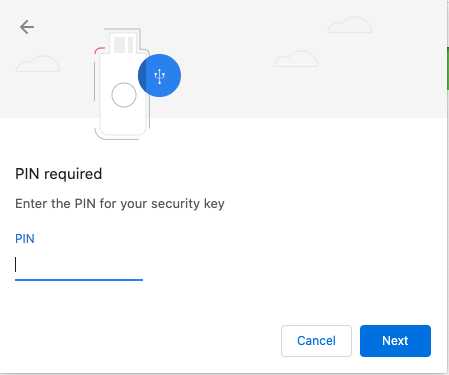
\includegraphics[width=\linewidth]{Figs/webauthn-registration-dialog2.png}\\
 {\footnotesize PINの入力要求}
\end{minipage}
\end{tabular}
\end{frame}

\begin{frame}[fragile]
この流れは、Shellからサンプルコードのディレクトリで以下を実行すると確認できる。
\begin{exampleblock}{\footnotesize ユーザ登録→ユーザ認証の一連のテストコードを実行}
{\footnotesize
\begin{verbatim}
$ yarn test
\end{verbatim}
}
\end{exampleblock}

\vspace{2ex}
ブラウザにダイアログが出たところで認証\footnote[frame]{\scriptsize Security Key by Yubicoの場合はPIN入力+タッチ}を行えば、\alert{認証器内部でCredentialが生成\&出生証明される。}

\vspace{2ex}
それでは、次のCredential生成ステップと、生成したCredentialの中身を覗いてみよう。
\end{frame}

\begin{frame}{WebAuthn ユーザ登録: Credential生成・取り出し}
\small
④,⑤ 認証器でCredential新規生成、Credential Public Keyと署名を取得。
\begin{center}
 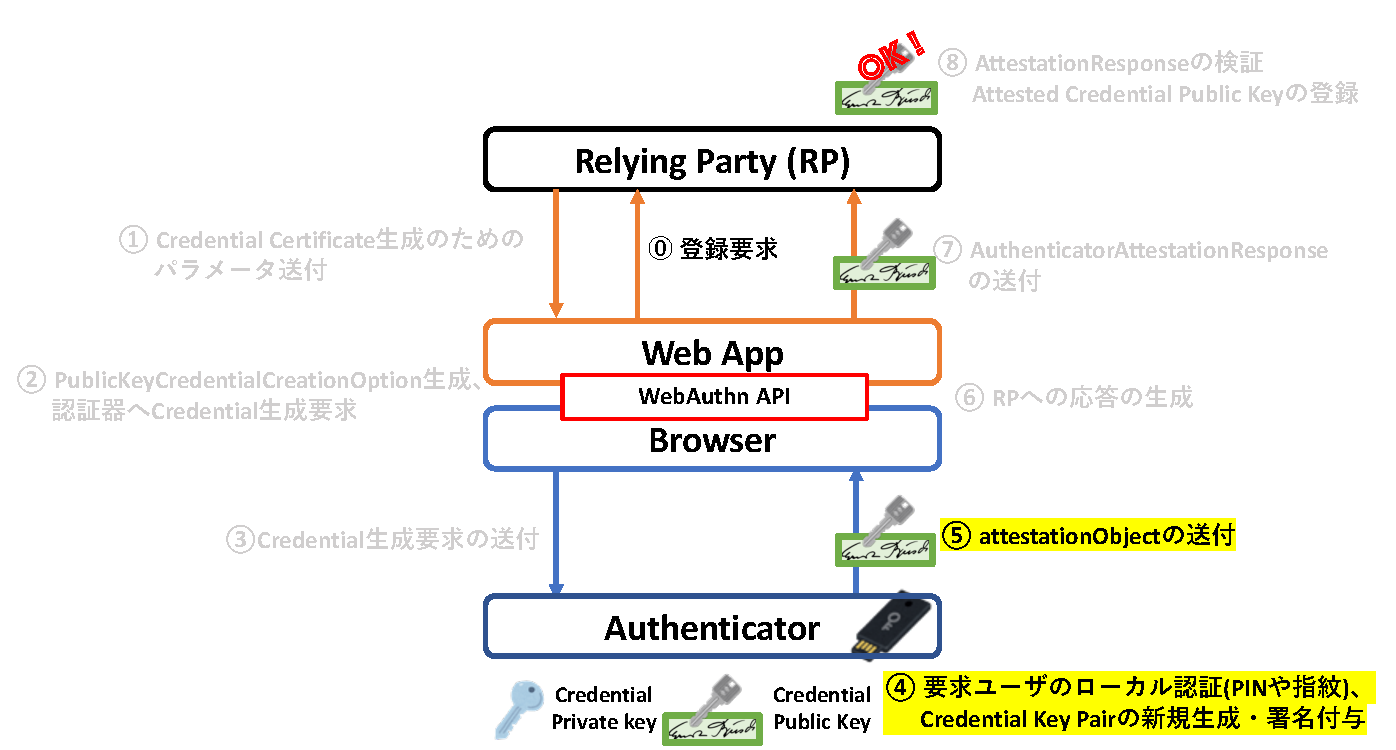
\includegraphics[width=0.9\linewidth]{Figs/webauthn-registration3.pdf}
\end{center}
前ステップの\texttt{create()}の返り値として、Attestation CertifiateやCredential Public Key (\texttt{attestationObject})を格納した\texttt{PublicKeyCredential} Objectをブラウザが取得。
\end{frame}

\begin{frame}
\small
\textbf{④-1: ローカルでの生体認証}\\[2ex]

前ステップの後、認証器ローカルでの生体認証\footnote[frame]{\scriptsize Security Key by Yubicoの場合、PIN入力の後にタッチすること。}、およびFIDO2 WebAuthnの利用確認が求められる。

\vspace{2ex}

\begin{tabular}{ccc}
\begin{minipage}{0.4\linewidth}
 \centering
 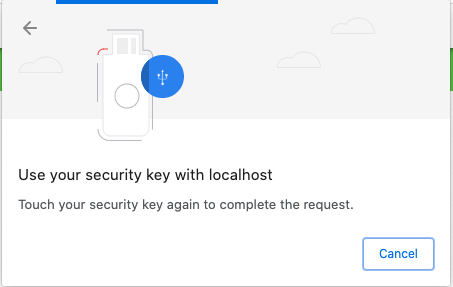
\includegraphics[width=\linewidth]{Figs/webauthn-registration-dialog3.png}\\
 {\footnotesize 認証要求}
\end{minipage}
 &
$\Rightarrow$
&
\begin{minipage}{0.4\linewidth}
 \centering
 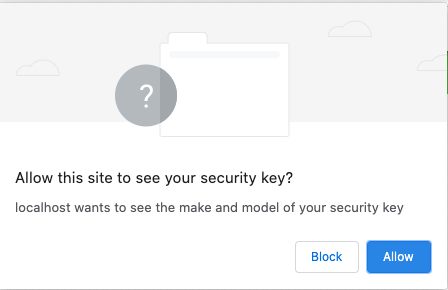
\includegraphics[width=\linewidth]{Figs/webauthn-registration-dialog4.png}\\
 {\footnotesize FIDO2利用意思の確認}
\end{minipage}
\end{tabular}
\end{frame}

\begin{frame}
\textbf{④-2: Credential Key Pairの新規生成・署名付与}\\[2ex]

\small
認証と利用意思確認が完了すると、認証器内部で以下の処理を実行。
\begin{enumerate}
\setlength{\itemsep}{0ex}
 \item ローカルでの生体認証結果の確認
 \item \texttt{create()}で入力されたパラメタに応じて、ユーザの新しい鍵ペア `Credential Key Pair' を生成
 \item 認証器内部のAttestation Private KeyでCredential Public Keyに署名
 \item (Attested) Credential Public Keyとその署名を出力\footnote[frame]{\scriptsize Attestation Type: directの場合はAttestation Certificateも出力}
\end{enumerate}
\begin{center}
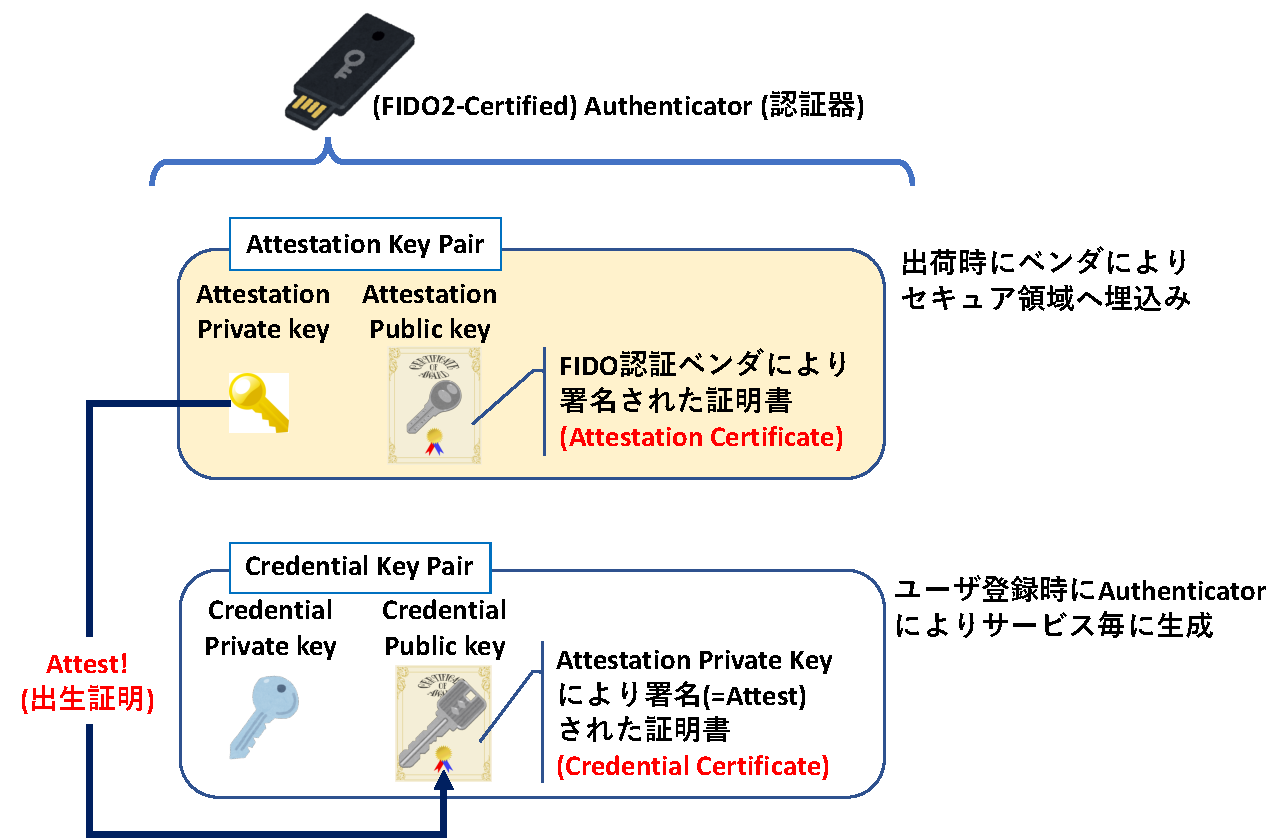
\includegraphics[width=0.5\linewidth]{Figs/webauthn-attestation.pdf}
\end{center}
\end{frame}

\begin{frame}[fragile]
\small
\textbf{⑤: ブラウザにて\texttt{PublicKeyCredential}の取得}\\[2ex]

\texttt{create()}の返り値 \texttt{PublicKeyCredential} Objectは単純に以下の4つの要素で構成されている。
\begin{exampleblock}{\scriptsize PublicKeyCredentialの構造 (\texttt{\$ yarn test}の途中出力)}
{\tiny
\begin{verbatim}
'------ [Response from Authenticator: PublicKeyCredential] ------'
'> Credential ID: HfM8J_xY7mn7bfiHxF7f7MLxf...' ← 生成した公開鍵のID
'> Credential Raw ID: [object ArrayBuffer]'     ← 生成した公開鍵のIDのバイナリ版
'> Credential Type: public-key'                 ← 公開鍵証明書なので'public-key'
'> AuthenticatorAttestationResponse.clientDataJSON: [object ArrayBuffer]'   ← RPのChallengeの情報 (バイナリ)
'> AuthenticatorAttestationResponse.attestationObject: [object ArrayBuffer]'← ここがCredential Public Keyと署名が含まれる本体 (バイナリ)
\end{verbatim}
}
\end{exampleblock}

このうち、「\texttt{clientDataJSON}」と「\texttt{attestationObject}」からなる\texttt{AuthenticatorAttestationResponse}をRPに送って検証・登録する。次のステップでその検証について解説する。


\end{frame}

\begin{frame}{WebAuthn ユーザ登録: Attestationの検証}
⑥,⑦,⑧ ブラウザが\texttt{AuthenticatorAttestationResponse}をRPに送って、そこでAttestationの検証とユーザ登録を実行。
\begin{center}
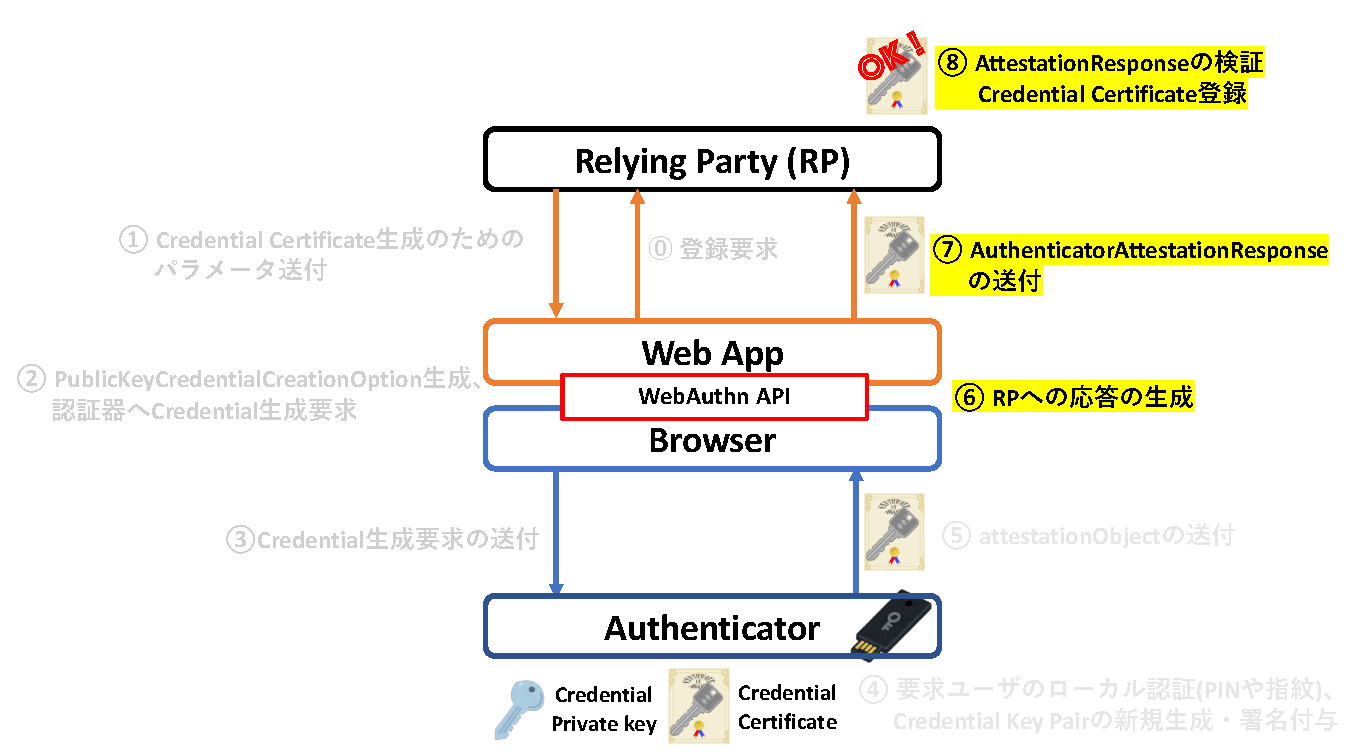
\includegraphics[width=0.9\linewidth]{Figs/webauthn-registration4.pdf}
\end{center}
\alert{Attestationの検証はRPの行うバックエンドの処理なことに注意。}
\end{frame}

\begin{frame}[fragile]
\textbf{⑥: ブラウザにて認証器出力をパース、RPへの応答を作成}\\
\textbf{⑦: \texttt{attestationObject}と\texttt{clientdataJSON}をRPへ送付}\\[2ex]

\texttt{clientDataJSON}はバイナリにエンコードされたJSONで、以下の要素で構成。
\begin{exampleblock}{\footnotesize \texttt{clientDataJSON}\footnote[frame]{\tiny WebAuthnの認証の時もパラメータの異なるこのオブジェクトが生成される。\url{https://developer.mozilla.org/en-US/docs/Web/API/AuthenticatorResponse/clientDataJSON}}の構造。 (\texttt{\$ yarn testの途中結果})}
\tiny
\begin{verbatim}
LOG: '------ [Decoding result of elements of AuthenticatorAttestationResponse] ------'
LOG: '> Decoded clientDataJSON:
{
  "challenge": "o9sKvn8ls2QAMFNyiv_g...", ← 登録処理開始の際、RPが送付したchallenge (base64url)。
  "origin": "http://localhost:9876",      ← Relying partyのID。今回の例だとlocalhost。
  "type": "webauthn.create"               ← ユーザ登録のときはwebauthn.create固定。
}'
\end{verbatim}
他、\texttt{tokenBindingId}というRPとの通信セッションとの紐付けを行うパラメタ (Optional)。
\end{exampleblock}
これは、\textbf{後述する\texttt{attstationObject}がどういうパラメタに対して生成されたのかを示す}一覧という位置づけ。
\end{frame}

\begin{frame}[fragile]
\small
\texttt{attestationObject}はCBOR\footnote[frame]{\tiny Concise Binary Object Representation。バイナリのJSONのようなもの。}で表現され、以下の要素で構成。

\vspace{-1ex}

\begin{exampleblock}{\footnotesize \texttt{attestationObject}\footnote[frame]{\tiny \texttt{clientDataJSON}と異なり、登録の時のみ生成されるオブジェクト。}の構造。 (\texttt{\$ yarn testの途中結果})}
{\tiny
\begin{verbatim}
[
  {
    "fmt": "packed",                      ← フォーマット規定。WebAuthnの場合は"packed"で最適化されている。
    "attStmt": {                          /* fmt="packed"のとき、Attestation Certificateと署名のフィールド */
      "alg": -7,                          ← ECDSA with SHA-256で作られた署名という意味 (COSE)
      "sig": {
        "type": "Buffer",
        "data": "MEUCIBJog73SH9q+gu...",  ← "x5c"の証明書で検証可能な署名 (本当はバイナリ)
      },
      "x5c": [
        {
          "type": "Buffer",
          "data": "MIICvDCCAaSgAwIB...",  ← これこそがAttestation Certificate!
        }
      ]
    },
    "authData": {                         /* 署名対象、つまりCredential Public Keyのフィールド */
      "type": "Buffer",
      "data": "SZYN5YgOjGh0NBcPZHZg..."   ← Credential Public Keyとそのメタ情報(登録するRPのIDなど)、
                                             ローカル生体認証の結果など (本当はバイナリ)
    }
  }
]'
\end{verbatim}
}
\end{exampleblock}
\vspace{-1ex}

{\footnotesize
fmt=``packed''の場合、\textbf{署名は、\texttt{clientDataJSON}のハッシュ値と、\texttt{attestationObject.authData}を連結したデータに対して生成。}}
\end{frame}

\begin{frame}
\small
\textbf{⑧: RPによる検証・登録}\\[2ex]

RPは\texttt{attestationObject}と\texttt{clientDataJSON}について以下を検証。

\begin{enumerate}
 \item \textbf{RP自身が要求したCredential生成なのか?}\\
$\Rightarrow$ \texttt{clientDataJSON}内部と、RPで保持していたチャレンジの比較
 \item \textbf{RPのサービスで登録すべきCredential生成なのか?}\\
\begin{itemize}
 \item[$\Rightarrow$] \texttt{clientDataJSON}内部のoriginのチェック
 \item[$\Rightarrow$] \texttt{attestationObject.authData}に含まれるRP IDのチェック
\end{itemize}
 \item \textbf{FIDO2で利用可能な正しい認証器を使った登録か?}\\
\begin{itemize}
 \item[$\Rightarrow$] \alert{\texttt{clientDataJSON}のハッシュ値と\texttt{authData}について、\texttt{attStmt.sig} (署名) の正しさを\texttt{attStmt.x5c} (Attestation Certificate) を使って検証}
 \item[$\Rightarrow$] \alert{ルート証明書により、\texttt{attStmt.x5c} の信頼性を検証}
\end{itemize}

\end{enumerate}
上記のチェックが全部OKであれば\texttt{authData} (内部のAttested Credential Public Key) を保存、ユーザ登録完了!
\end{frame}

\begin{frame}[fragile]
\small
テストコードで模擬するRPのAttestation検証動作結果を見てみよう。
\begin{exampleblock}{\scriptsize RPによるPublicKeyCredentialの検証結果の例 (\texttt{\$ yarn test}の途中出力)}
\tiny
 \begin{verbatim}
LOG: '------ [Verification result on PublicKeyCredential.AuthenticatorAttestationResponse] ------'
LOG: '> Verification result: true'      ← Attestationの検証成功 (challenge/origin/署名の検証成功)

LOG: '> Attested Credential Public Key: ← 検証が成功した Attested Credential Public Key (毎回変化; これを登録)
-----BEGIN PUBLIC KEY-----
MFkwEwYHKoZIzj0CAQYIKoZIzj0DAQcDQgAEt11IqJnVr2Wi4nIip57LPhoAejRG
TH86zg3S7CUYSFibLqVOQrbQ00ADz9IpYHoKzQCbbHcl3o8Zj7WgHUy1yQ==
-----END PUBLIC KEY-----'

LOG: '> Attestation Certificate:        ← 認証器が送ってきたAttestation Certificate (固定)
-----BEGIN CERTIFICATE-----
MIICvDCCAaSgAwIBAgIEBMX+/DANBgkqhkiG9w0BAQsFADAuMSwwKgYDVQQDEyNZ
dWJpY28gVTJGIFJvb3QgQ0EgU2VyaWFsIDQ1NzIwMDYzMTAgFw0xNDA4MDEwMDAw
MDBaGA8yMDUwMDkwNDAwMDAwMFowbTELMAkGA1UEBhMCU0UxEjAQBgNVBAoMCVl1
YmljbyBBQjEiMCAGA1UECwwZQXV0aGVudGljYXRvciBBdHRlc3RhdGlvbjEmMCQG
A1UEAwwdWXViaWNvIFUyRiBFRSBTZXJpYWwgODAwODQ3MzIwWTATBgcqhkjOPQIB
BggqhkjOPQMBBwNCAAQc2Np2EaP17x+IXpULpl2A4zSFU5FYS9R/W3GcUyNcJCHk
45m9tXNngkGQk1dmYUk8kUwuZyTfk5T8+n3qixgEo2wwajAiBgkrBgEEAYLECgIE
FTEuMy42LjEuNC4xLjQxNDgyLjEuMTATBgsrBgEEAYLlHAIBAQQEAwIFIDAhBgsr
BgEEAYLlHAEBBAQSBBD4oBHzjApNFYAGFxEfntx9MAwGA1UdEwEB/wQCMAAwDQYJ
KoZIhvcNAQELBQADggEBAHcYTO91LRoF8wpThdwthvj6wGNxcLAiYqUZXPX+0Db+
AGVODSkVvEVSmj+JXmrBzNQel3FW4AupOgbgrJmmcWWEBZyXSpRQtYcl2LTNU0+I
z9WbyHNN1wQJ9ybFwj608xBuoNRC0rG8wgYbMC4usyRadt3dYOVdQi0cfaksVB2V
NKnw+ttQUWKoZsPHtuzFx8NlazLQBep1W2T0FCONFEG7x/l+ZcfNhT13azAbaurJ
2J0/ff6H0PXJP6h+Obne4xfz0+8ujftWDUSh9oaiVRYf+tgam/tzOKyEU38V2liV
11zMyHKWrXiK0AfyDgb58ky2HSrn/AgE5MW/oXg/CXc=
-----END CERTIFICATE-----'
\end{verbatim}
\end{exampleblock}
署名検証のソースコード解説は、ただのフォーマット解説のため省略。
\end{frame}


\subsection{WebAuthn ユーザ認証フロー}

\begin{frame}
\centering
{\Large FIDO2 WebAuthn ユーザ認証フロー}
\end{frame}

\begin{frame}{WebAuthn ユーザ認証フロー}
以下のような流れで、RPに登録されたユーザに対し、認証を行う。
\begin{center}
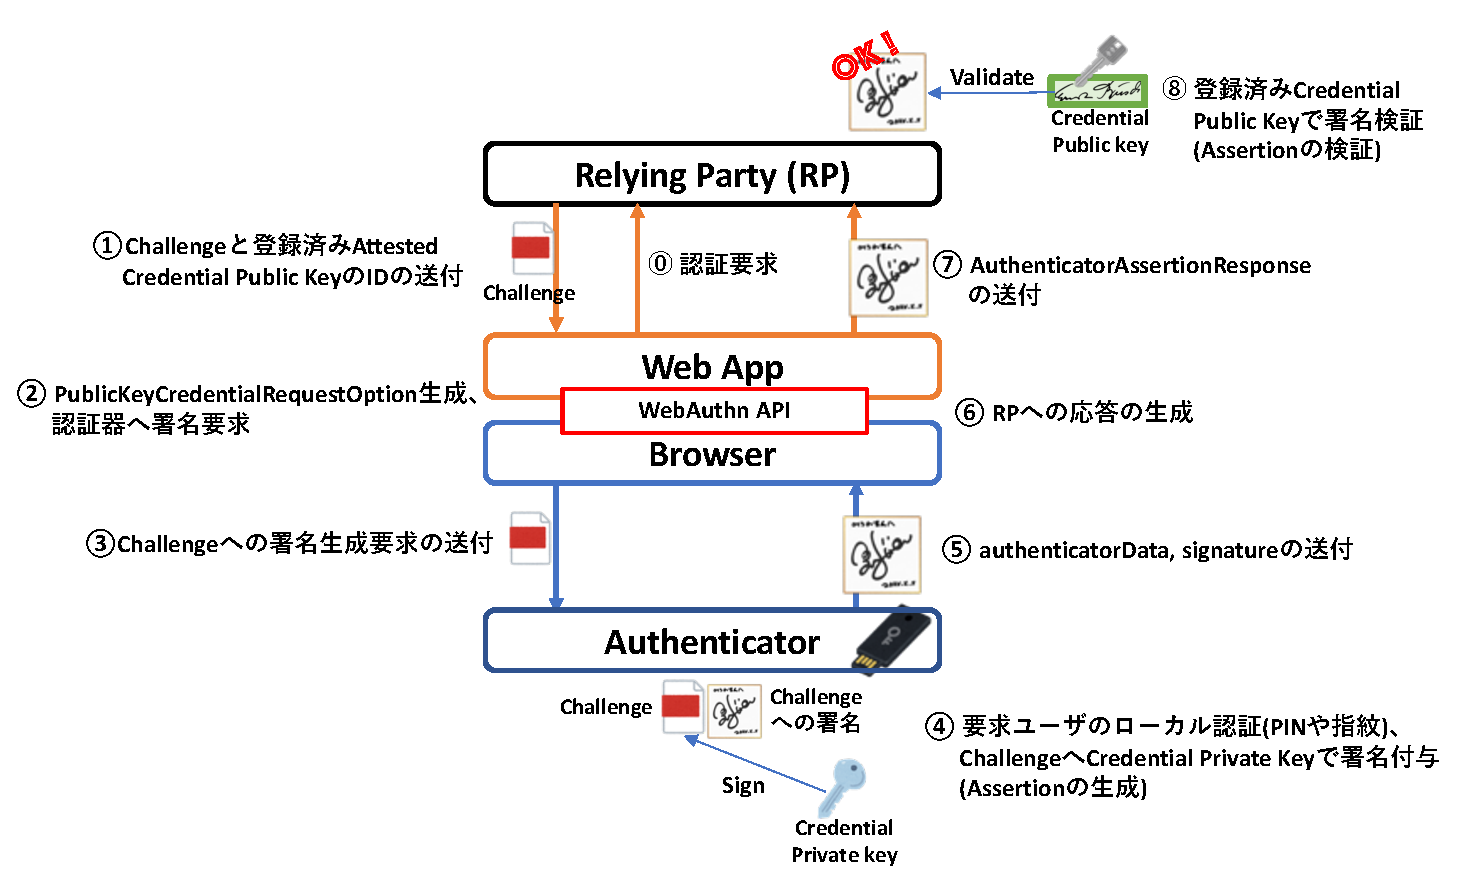
\includegraphics[width=0.9\linewidth]{Figs/webauthn-authentication0.pdf}
\end{center}
RPで生成した\textbf{Challengeに対して認証器内部で署名}させ、その検証結果で事前に登録したユーザかどうかを判別・認証する処理。
\end{frame}

\begin{frame}
登録処理の場合同様、ユーザ認証の各ステップを実際のデータを確認しながら追っていく。

\begin{block}{\small ``Assertion''について}
ユーザ登録の時、Credential (Key Pair)の「認証器による出生証明」を``Attestation''と呼んだ。
これと同様に\alert{FIDO2 WebAuthnでは、ユーザ認証において「認証器による正当性の主張」を``Assertion''と呼ぶ}。
すなわち、\textbf{Assertionの検証を行うことで、RPは正当性の主張を受入れ認証OKとする}。
\end{block}
\end{frame}

\begin{frame}{WebAuthn ユーザ認証: RPへユーザ認証要求}
\begin{center}
⓪,① Challengeと署名させるCredentialのIDをRPから取得。
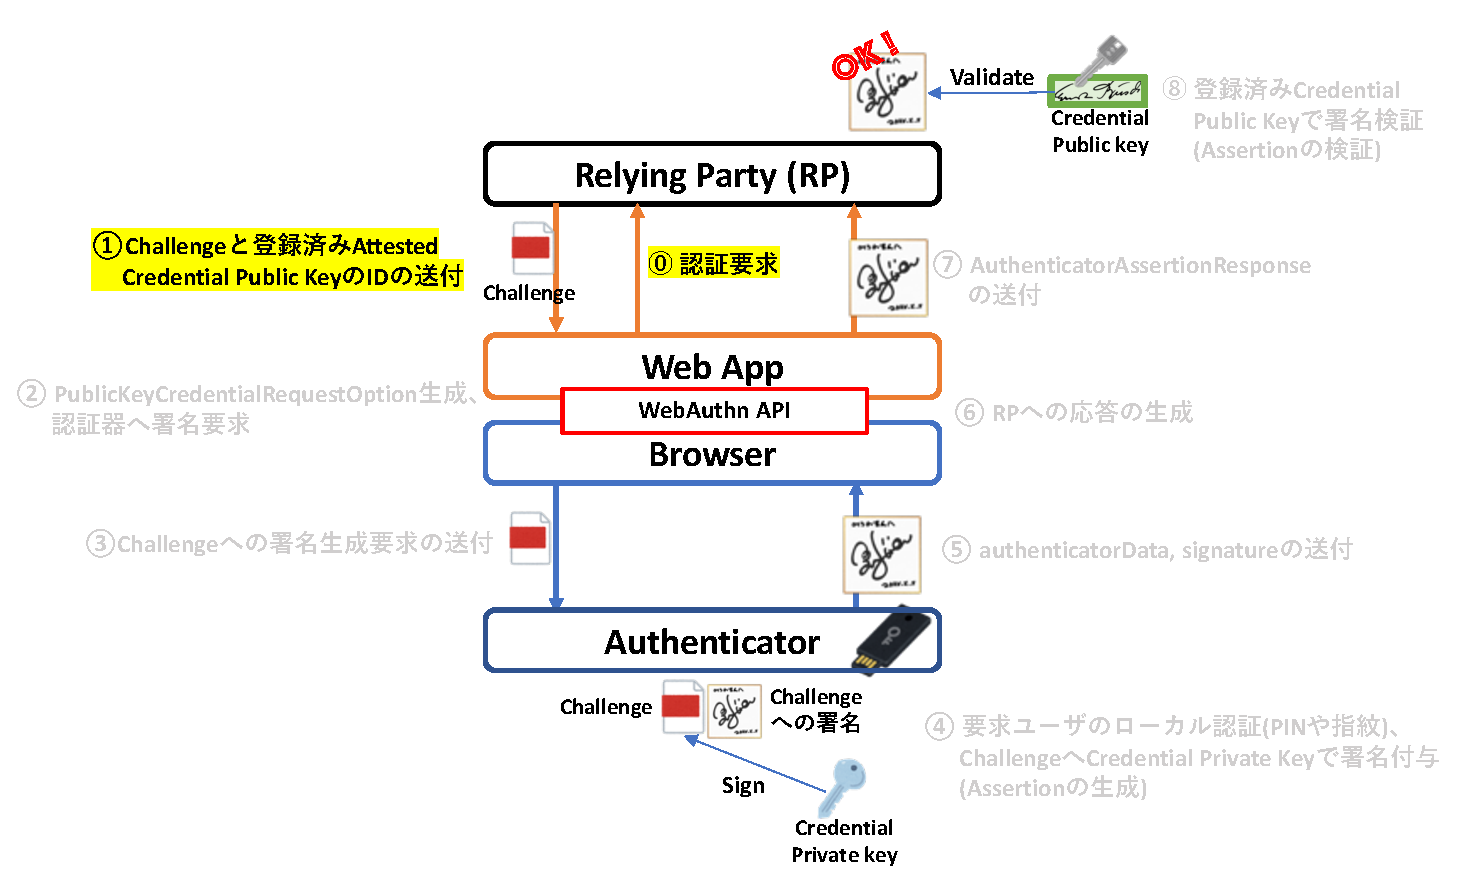
\includegraphics[width=0.9\linewidth]{Figs/webauthn-authentication1.pdf}
\end{center}
登録同様、WebApp・RP間のやりとりは規定されておらず、実装者に任されている。
\end{frame}

\begin{frame}
WebAppがRPから取得する必要があるパラメタは以下の通り。
\begin{itemize}
 \item \textbf{Challenge}: \alert{暗号学的にランダムな使い捨てのbinary string (最低16bytes, 通常32bytes程度)}
 \item \textbf{Credential Info}: ユーザのCredential Public KeyのID。認証器に対応するCredential Private Key (署名鍵) を指定するのに必要。規格上はOptionalだが\alert{認証器が非対応の場合は指定が必須。}\footnote[frame]{\scriptsize Client-side Discoverable Credential (後述) に対応していることが必要。Security Key by Yubicoは非対応。}
\end{itemize}

\vspace{2ex}

ブラウザはこれらを\texttt{PublicKeyCredentialRequestOptions} Objectにし、WebAuthn API経由で認証器へAssertionを要求。
\end{frame}


\begin{frame}{WebAuthn ユーザ認証: 認証器へAssertion生成要求}
②,③ ブラウザのAPIを通して認証器へAssertionを要求。
\begin{center}
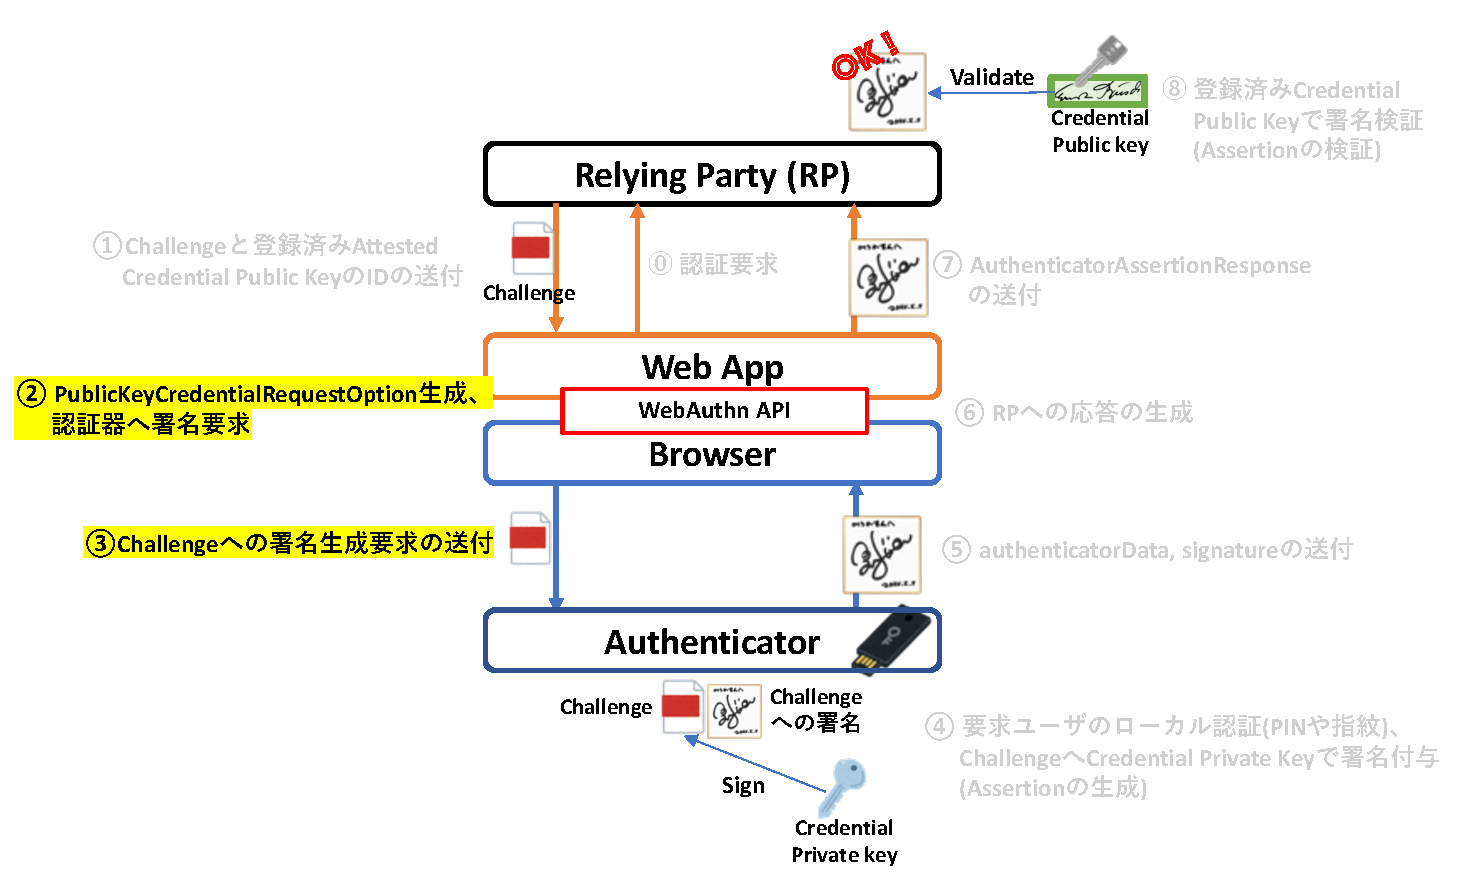
\includegraphics[width=0.9\linewidth]{Figs/webauthn-authentication2.pdf}
\end{center}
\texttt{PublicKeyCredentialRequestOptions} Objectをブラウザの\texttt{window.navigator.credential.get()}へ入力。
\end{frame}

\begin{frame}[fragile]
\textbf{②: 認証器に送るオブジェクトの生成}\\[2ex]
実際にJavaScriptのコードを見ていく。
\begin{exampleblock}{\scriptsize \texttt{PublicKeyCredentialRequestOptions}の構造 (\texttt{./test/credential-params.ts})}
\tiny
\begin{verbatim}
export const getCredentialDefaultArgs: CredentialRequestOptions = {
  publicKey: {
    // Challenge 本当はサーバーで生成した暗号学的に安全な乱数をセット (16bytes以上)
    challenge: new Uint8Array([
      0x79, 0x50, ...
    ]).buffer,

    // Info of credential public keys allowed to use authentication (optional)
    // 認証器次第ではここをRPが指定しなくてもOK
    // (RP IDに応じてユーザが鍵を選べる, Client-side Discoverable Credentialと呼ぶ)
    allowCredentials: [{
      id: new Uint8Array([0xA1, 0x55, ...]).buffer,
      transports: ['usb', 'nfc', 'ble'],
      type: 'public-key'
    }],

    // rpId indicating Relying Party ID (optional, default = current domain)
    rpId: 'localhost', // テストコードはローカルで走るため

    // User verification (biometrics authentication, optional, default = 'preferred')
    // PINが未指定の場合などは、'required'にすると検証不可として認証エラー
    userVerification: 'required',

    // Time out (optional, in msec)
    timeout: 60000,
  },
};
\end{verbatim}
\end{exampleblock}
 
\end{frame}

\begin{frame}[fragile]
\small
\textbf{③: 認証器へオブジェクト送付}\\[2ex]

\texttt{PublicKeyCredentialRequestOptions} Objectを使ってブラウザのWebAuthn APIを以下のようにCallすると、登録の時と同様に認証器の挿入・接続要求、\alert{PIN入力要求、認証要求がブラウザ通知}される。

\begin{exampleblock}{\scriptsize \texttt{window.navigator.credential.get()}のCall (\texttt{./test/test.spec.ts})}
{\scriptsize
\begin{verbatim}
const cred: Credential|null
  = await window.navigator.credentials.get(getCredentialDefaultArgs);
\end{verbatim}
}
\end{exampleblock}
\end{frame}


\begin{frame}
\begin{exampleblock}{\footnotesize 補足: Client-side Discoverable Credentialについて}
\small
\texttt{PublicKeyCredentialRequestOptions}において、\texttt{allowCredentials}なしとするClient-side Discoverable Credential\footnote[frame]{\scriptsize 現在の仕様(ver. 4 Mar. 2019)上はResident Credentialと呼ばれているが、Working Draftで名称が変わった。\url{https://w3c.github.io/webauthn/\#client-side-discoverable-credential}}が利用できる。
この機能は、以下の特徴を持つ。
\begin{itemize}
\item 認証時にRPからCredential IDを取得する必要がなく、ユーザ自身がRP IDに応じてCredentialを切り替え可能
\item RP側でユーザ名などとCredential IDの紐付け管理が不要
\end{itemize}
ただし、利用には\structure{認証器がこの機能に対応している必要}がある。
\end{exampleblock}
\end{frame}


\begin{frame}{WebAuthn ユーザ認証: Assertion生成・取り出し}
\small
④,⑤ 認証器でChallengeへ署名し、Assertionを取得。
\begin{center}
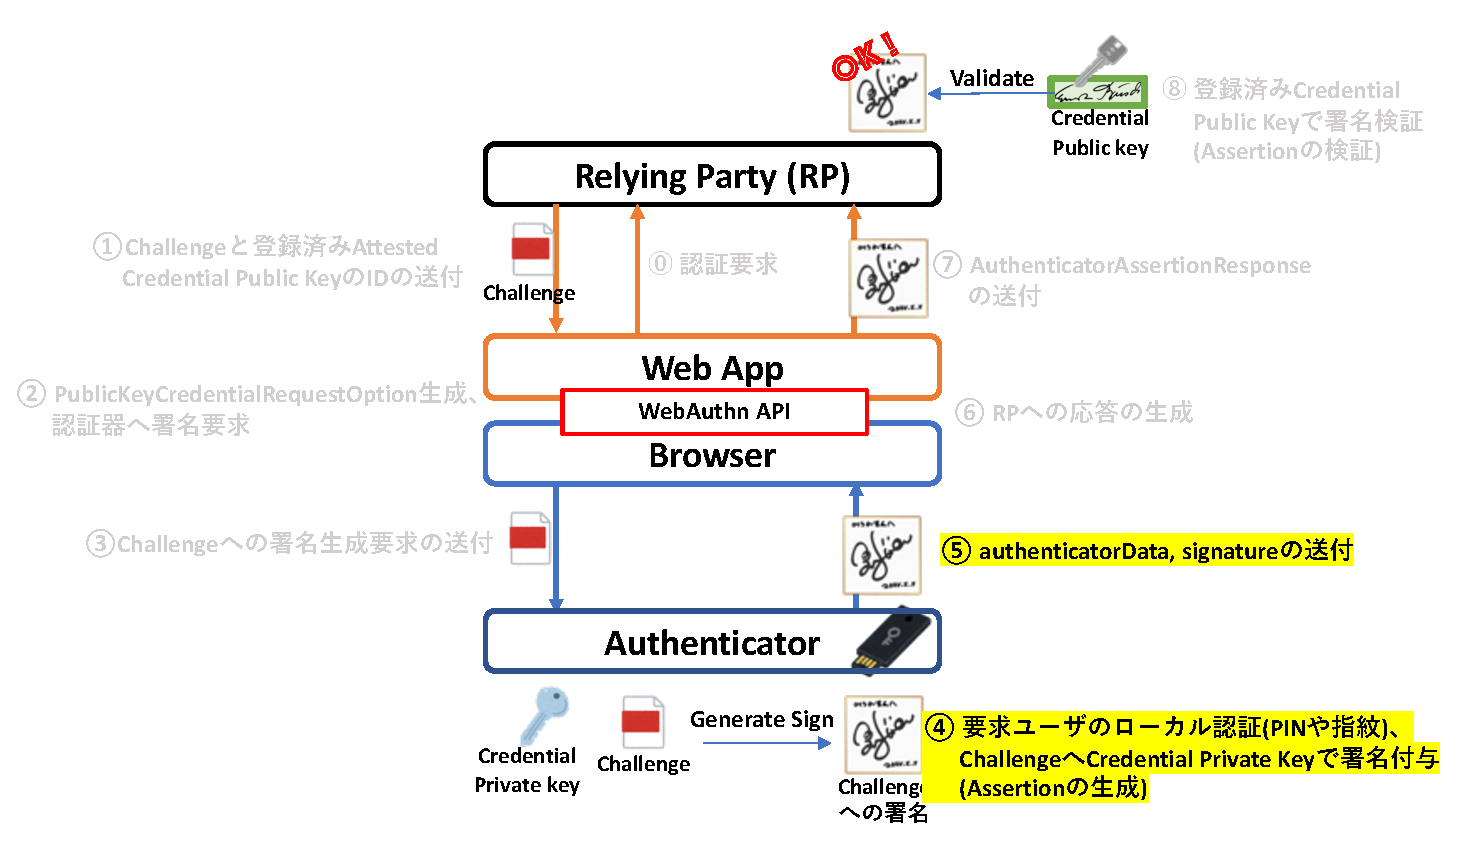
\includegraphics[width=0.9\linewidth]{Figs/webauthn-authentication3.pdf}
\end{center}
前ステップの\texttt{get()}の返り値として、署名(\texttt{signature})やメタ情報(\texttt{authenticatorData})を格納した\texttt{PublicKeyCredential} Objectを取得。
\end{frame}

\begin{frame}
\textbf{④: ローカルでの生体認証・認証器でのAssertion生成}\\[2ex]

認証器にタッチすることで生体認証を完了させると、\alert{認証器内部でAssertion = Challengeへの署名生成が行われる。}

\begin{center}
\begin{tabular}{ccc}
\begin{minipage}{0.4\linewidth}
 \centering
 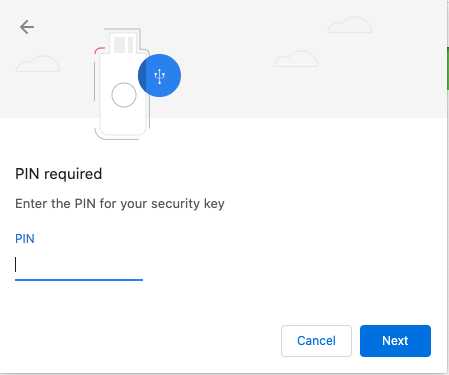
\includegraphics[width=\linewidth]{Figs/webauthn-registration-dialog2.png}\\
 {\footnotesize PIN入力要求}
\end{minipage}
 &
$\Rightarrow$
&
\begin{minipage}{0.4\linewidth}
 \centering
 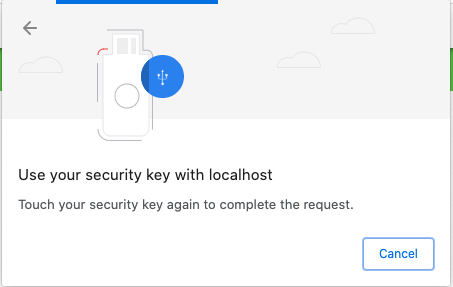
\includegraphics[width=\linewidth]{Figs/webauthn-registration-dialog3.png}\\
 {\footnotesize 認証要求}
\end{minipage}
\end{tabular}
\end{center}
\end{frame}

\begin{frame}[fragile]
\small
\textbf{⑤: ブラウザにて\texttt{PublicKeyCredentialObject}の取得}\\[2ex]

\texttt{get()}の返り値 \texttt{PulicKeyCredential} Objectは以下の要素で構成される。\texttt{create()}では\texttt{AuthenticatorAttestationResponse}が入っていたが、\alert{\texttt{AuthenticationAssertionResponse}が入ることに注意。}

\begin{exampleblock}{\footnotesize PublicKeyCredentialの構造 (\texttt{\$ yarn test}の途中出力)}
\tiny
\begin{verbatim}
LOG: '------ [Response from Authenticator: PublicKeyCredential] ------'
LOG: '> Credential ID: jsQqwn1tT5C-I01ELUVq7m...'     ← 署名検証に用いる公開鍵のID = Credential Public Key ID
LOG: '> Credential Raw ID: [object ArrayBuffer]'      ← IDのバイナリ版
LOG: '> Credential Type: public-key'                  ← 署名は公開鍵で検証されるものなので'public-key'
LOG: '> AuthenticatorAssertionResponse.clientDataJSON: [object ArrayBuffer]'   ← RPのChallengeの情報
LOG: '> AuthenticatorAssertionResponse.authenticatorData: [object ArrayBuffer]'← 認証器の情報やRPのIDなど
LOG: '> AuthenticatorAssertionResponse.signature: [object ArrayBuffer]'        ← RPのChallengeに対する応答=署名!
LOG: '> AuthenticatorAssertionResponse.userHandle: null'                       ← Create時に入力したユーザIDが入ることが多い
\end{verbatim}
\end{exampleblock}

このうち、\texttt{AuthenticatorAssertionResponse}内部の4要素をRPに送って検証 (Assertionの検証)、認証可否を判断する。次ステップでその手順を解説する。
\end{frame}



\begin{frame}{WebAuthn ユーザ認証: Assertionの検証}
\small
⑥,⑦,⑧ ブラウザが\texttt{AutehtncatorAssertionResponse}をRPへ送って、そこでAssertionの検証と認証可否判断を行う。
\begin{center}
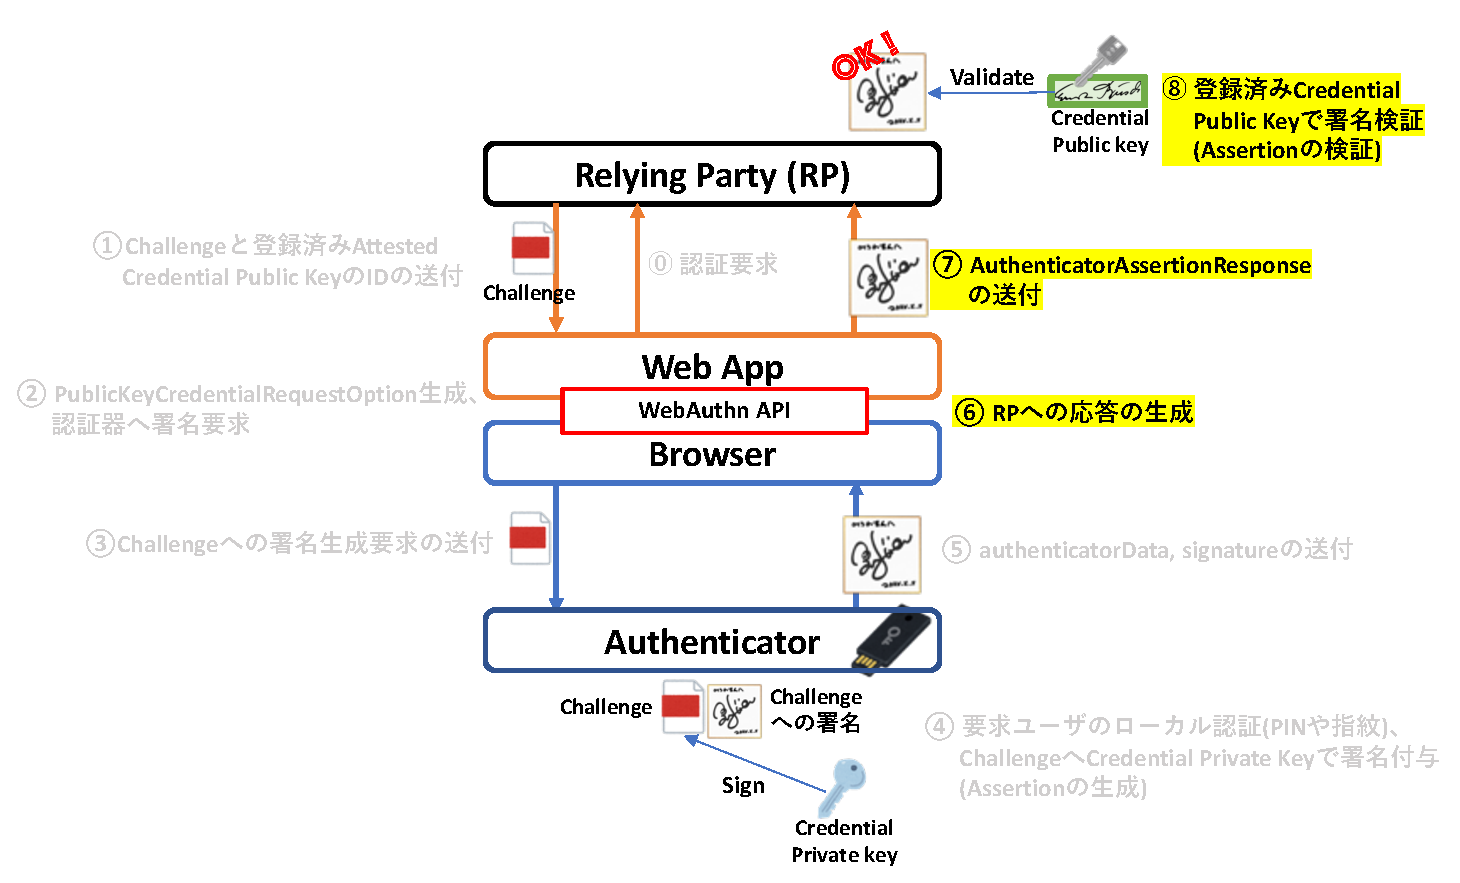
\includegraphics[width=0.9\linewidth]{Figs/webauthn-authentication4.pdf}
\end{center}
\alert{Assertionの検証はRPの行うバックエンドの処理なことに注意。}
\end{frame}

\begin{frame}[fragile]
\small 
\textbf{⑥: ブラウザにて認証器出力をパース、RPへの応答を作成}\\
\textbf{⑦: \textbf{clientDataJSON}・\textbf{authenticatorData}・\textbf{signature}をRPへ送付}\\[2ex]

\texttt{AuthenticatorAssertionResponse}の要素の構造は以下の通り。

\begin{exampleblock}{\scriptsize \texttt{clientDataJSON}の構造, \texttt{authenticatorData}, \texttt{signature} (\texttt{\$ yarn test}の途中結果)}
\tiny
\begin{verbatim}
LOG: '------ [Decoding result of elements of AuthenticatorAssertionResponse] ------'
LOG: '> Decoded clientDataJSON: {
  "challenge": "rHNRQ6copASyNLyFv0Ja...", ← 認証処理開始の際、RPが送付したchallenge (base64url)
  "origin": "http://localhost:9876",      ← RP ID
  "type": "webauthn.get"                  ← ユーザ認証の時はwebauthn.get固定。
}'


LOG: '> Base64 authenticatorData: SZYN5YgOj...' ← 認証器の情報やCredentialが紐付けられているRP IDなどのデータ


LOG: '> Base64 signature: MEYCIQDI0cKyqpksA...' ← clientDataJSONとauthenticatorDataに対して作られた署名
\end{verbatim}
\end{exampleblock}
\textbf{clientDataJSONのハッシュ値とauthenticatorDataを連結したデータに対してCredential Private Keyで署名生成}されている。

\vspace{1ex}

$\Rightarrow$ RPはこの連結データに対してsignatureが正しいものかどうかを検証。
\end{frame}

\begin{frame}
\textbf{⑧: RPによる検証・認証可否の決定}
\small
RPは\texttt{authenticatorData}、\texttt{signature}、\texttt{clientDataJSON}に対して以下を検証する。(=\alert{Assertionの検証})
\begin{enumerate}
 \item \textbf{RP自身が要求したAssertion作成なのか?}\\
$\Rightarrow$ \texttt{clientDataJSON}内部と、RPで保持していたチャレンジの比較
 \item \textbf{RPのサービスで認証すべき要求なのか?}\\
\begin{itemize}
 \item[$\Rightarrow$] \texttt{clientDataJSON}内部のoriginのチェック
 \item[$\Rightarrow$] \texttt{authenticatorData}に含まれるRP IDのチェック
\end{itemize}
 \item \textbf{事前登録したユーザ・認証器によって作られたAssertionか?}\\
$\Rightarrow$ Credential IDが紐づいているAttested Credential Public Keyを登録ユーザのDBから取得。\alert{\texttt{clientDataJSON}のハッシュ値と\texttt{authenticatorData}について、\texttt{signature} (署名) の正しさを、Credential Public Keyで検証。}
\end{enumerate}
\end{frame}


\begin{frame}[fragile]
テストコードで模擬するRPのAssertion検証結果を見てみよう。
\begin{exampleblock}{\scriptsize assertion検証結果 (\texttt{\$ yarn test}の途中結果)}
\tiny
\begin{verbatim}
LOG: '------ [Verification result on PublicKeyCredential.AuthenticatorAssertionResponse] ------'
LOG: '> Verification result: true' ← Assertionの検証成功 (challenge/origin/署名の検証成功)
\end{verbatim}
\end{exampleblock}
Assertion検証のソースコード解説は、ただのフォーマット解説のため省略。
\end{frame}

\section{まとめ}
\begin{frame}
\centering
{\huge まとめ}
\end{frame}

\begin{frame}
この資料では以下を行った。
\begin{itemize}
 \item 認証の基礎と、FIDO2の概要の紹介
 \item FIDO2 WebAuthnの概要の紹介
 \item FIDO2 WebAuthnのユーザ登録・認証についてコードレベルで動作解説
\end{itemize}

ただし、今回触ってみたことがWebAuthnの全体像ではないことに注意。仕様は日々進化しており、またパラメタもここで掲載したもの以外にも多く存在する。あくまで1つの例と考えてほしい。
\end{frame}


\begin{frame}{参考資料: WebAuthnの標準文書・仕様書}
\small
\begin{itemize}
 \item Web Authentication (W3C勧告)\\ \url{https://www.w3.org/TR/webauthn-1}
 \item Web Authentication (W3C Working Draft)\\ \url{https://w3c.github.io/webauthn}
 \item Web Authentication API (MDN)\\ \url{https://developer.mozilla.org/en-US/docs/Web/API/Web_Authentication_API}
\end{itemize}
\end{frame}


% %%%%%%%%%%%%%%%%%%%%%%%%%%%%%%%%%%%%%%%%%%%%%%%%%%%%%%%%%%%%%%%%%%%%%%%%%%%%%%%%%%%%%%%%%%%%%%%%%%%
% \backupbegin

% \section{Backup}

% \begin{frame}
 
% \end{frame}

% \begin{frame}
% \frametitle{Appendix}
% This page is not counted.
% \end{frame}
% \backupend
\end{document}
%%%%%%%%%%%%%%%%%%%%%%%%%%%%%%%%%%%%%%%%%%%%%%%%%%%%%%%%%%%%%%%%%%%%%%%%%%%%%%%%%%%%%%%%%%%%%%%%%%%
%%%%%%%%%%%%%%%%%%%%%%%%%%%%%%%%%%%%%%%%%%%%%%%%%%%%%%%%%%%%%%%%%%%%%%%%%%%%%%%%%%%%%%%%%%%%%%%%%%%
%%%%%%%%%%%%%%%%%%%%%%%%%%%%%%%%%%%%%%%%%%%%%%%%%%%%%%%%%%%%%%%%%%%%%%%%%%%%%%%%%%%%%%%%%%%%%%%%%%%
%%%%%%%%%%%%%%%%%%%%%%%%%%%%%%%%%%%%%%%%%%%%%%%%%%%%%%%%%%%%%%%%%%%%%%%%%%%%%%%%%%%%%%%%%%%%%%%%%%%
%%%%%%%%%%%%%%%%%%%%%%%%%%%%%%%%%%%%%%%%%%%%%%%%%%%%%%%%%%%%%%%%%%%%%%%%%%%%%%%%%%%%%%%%%%%%%%%%%%%
%%%%%%%%%%%%%%%%%%%%%%%%%%%%%%%%%%%%%%%%%%%%%%%%%%%%%%%%%%%%%%%%%%%%%%%%%%%%%%%%%%%%%%%%%%%%%%%%%%%
